% ============================================================
%  Chương 2: Thu thập kiến thức về quy định đào tạo
% ============================================================
\chapter{Thu thập kiến thức về quy định đào tạo}
\label{chap:chapter2}

Chương này trình bày tổng quan về hệ thống quy chế đào tạo thạc sĩ tại UIT và
ĐHQG-HCM, quy trình thu thập và tổ chức kiến thức từ các văn bản quy phạm, cùng
các công trình nghiên cứu liên quan đến bài toán thu thập kiến thức pháp lý.
Nội dung chương tuân theo phương pháp thu thập kiến thức theo miền (domain knowledge
acquisition) cho hệ thống truy xuất thông tin \cite{sartor2011legalonto}.

% ============================================================
\section{Giới thiệu về hệ thống quy chế đào tạo thạc sĩ}
\label{sec:gioithieu_quyche}

% ------------------------------------------------------------
\subsection{Tổng quan hệ thống quy chế đào tạo sau đại học tại Việt Nam}
\label{subsec:tongquan_hethong}

Hệ thống giáo dục sau đại học tại Việt Nam được quản lý bởi nhiều tầng văn bản quy
phạm pháp luật, từ cấp quốc gia đến cấp trường. Tại cấp quốc gia, Luật Giáo dục
(Luật số 43/2019/QH14) và Luật Giáo dục Đại học (Luật số 08/2012/QH13, sửa đổi bổ
sung bởi Luật số 34/2018/QH14) đặt ra khung pháp lý chung cho toàn bộ hệ thống giáo
dục. Bộ Giáo dục và Đào tạo ban hành các quy chế đào tạo trình độ thạc sĩ, tiến sĩ
áp dụng trên toàn quốc (Thông tư số 23/2021/TT-BGDĐT quy chế tuyển sinh và đào tạo
trình độ thạc sĩ). Tại cấp cơ sở, các đại học quốc gia và trường đại học ban hành
quy chế riêng phù hợp với đặc thù đào tạo, trong phạm vi quyền tự chủ được pháp
luật cho phép.

Mô hình quản trị này tạo ra một hệ thống quy chế phân tầng (layered regulation
system) với ba đặc điểm quan trọng ảnh hưởng đến bài toán truy xuất thông tin:

\begin{enumerate}
  \item \textbf{Tính phân cấp (Hierarchical):} Văn bản cấp trên đặt ra nguyên tắc
        chung, văn bản cấp dưới cụ thể hóa và bổ sung. Khi xảy ra mâu thuẫn, văn
        bản cấp trên có hiệu lực cao hơn. Ví dụ: QĐ~1393 (ĐHQG-HCM) quy định thời
        gian đào tạo tối đa 4 năm, QĐ~270 (UIT) cụ thể hóa thêm điều kiện gia hạn.

  \item \textbf{Tham chiếu chéo (Cross-reference):} Các điều khoản thường dẫn chiếu
        lẫn nhau, cả trong cùng văn bản (intra-document) và giữa các văn bản
        (inter-document). Ví dụ: Điều 24 QĐ~270 về điều kiện bảo vệ luận văn dẫn
        chiếu đến Điều 25 QĐ~1393 về yêu cầu ngoại ngữ đầu ra.

  \item \textbf{Thay thế và kế thừa (Succession):} Văn bản mới có thể thay thế toàn
        bộ hoặc sửa đổi bổ sung văn bản cũ. Ví dụ: QĐ~1393 (2021) thay thế QĐ~160
        (2017), nhưng học viên nhập học trước 2022 vẫn áp dụng QĐ~160 theo điều khoản
        chuyển tiếp.
\end{enumerate}

Đối với UIT, một trường thành viên của ĐHQG-HCM, hệ thống quy chế đào tạo thạc sĩ
bao gồm hai tầng chính:
\begin{itemize}
    \item \textbf{Tầng ĐHQG-HCM}: Các quy chế khung do ĐHQG-HCM ban hành, áp dụng
          cho tất cả các trường thành viên (QĐ~160, QĐ~1393, QĐ~218).
    \item \textbf{Tầng trường}: Các quy chế, quy định cụ thể hóa do UIT ban hành
          (QĐ~270, QĐ~851), bổ sung và chi tiết hóa các quy định của ĐHQG-HCM.
\end{itemize}

Mô hình hai tầng này đặt ra thách thức cho bài toán hỏi đáp: khi học viên hỏi về
một vấn đề cụ thể (ví dụ: ``điều kiện bảo vệ luận văn''), hệ thống cần kết hợp
thông tin từ cả hai tầng -- quy định chung từ ĐHQG-HCM và quy định bổ sung từ UIT
-- để đưa ra câu trả lời đầy đủ. Đây là một trong những động lực chính cho kiến
trúc truy xuất đa tầng được trình bày trong Chương~\ref{chap:thiet-ke-giai-thuat}.

% ------------------------------------------------------------
\subsection{Cấu trúc văn bản quy phạm}
\label{subsec:cautruc_vanban}

Các văn bản quy chế đào tạo tuân theo cấu trúc phân cấp chuẩn của văn bản quy phạm
pháp luật Việt Nam, được quy định trong Luật Ban hành văn bản quy phạm pháp luật
(Luật số 80/2015/QH13):

\[
\text{Văn bản} \rightarrow \text{Chương} \rightarrow \text{Mục} \rightarrow
\text{Điều} \rightarrow \text{Khoản} \rightarrow \text{Điểm}
\]

Mỗi cấp mang phạm vi pháp lý riêng biệt. Một Văn bản thường bao gồm nhiều
Chương, mỗi Chương có thể chứa các Mục gom nhóm các Điều theo chủ đề. Mỗi Điều
quy định về một vấn đề cụ thể và được chia thành các Khoản (đánh số 1, 2,
3\ldots) và Điểm (đánh số a, b, c\ldots). Trong thực tế, không phải văn bản nào
cũng có đủ cả 6 cấp; ví dụ các quy chế đào tạo thường không có cấp Mục.

Cấu trúc phân cấp này có ý nghĩa quan trọng cho bài toán truy xuất:

\begin{itemize}
  \item \textbf{Đơn vị trích dẫn (Citable unit):} Trong thực tiễn pháp lý và hành
        chính Việt Nam, đơn vị trích dẫn nhỏ nhất là Điểm hoặc Khoản (ví dụ: ``theo
        Điểm a Khoản 1 Điều 24 QĐ~270''). Tuy nhiên, Điều là đơn vị trích dẫn phổ
        biến nhất vì mỗi Điều thường quy định trọn vẹn một vấn đề.

  \item \textbf{Ngữ cảnh phân cấp (Hierarchical context):} Để hiểu đúng một Điều,
        cần biết nó thuộc Chương nào (xác định chủ đề tổng quát) và văn bản nào
        (xác định phạm vi hiệu lực và cấp ban hành).

  \item \textbf{Tham chiếu nội bộ (Internal reference):} Nhiều Điều sử dụng cụm từ
        như ``theo quy định tại Điều 5'' hoặc ``căn cứ Khoản 1 Điều 24'' để dẫn
        chiếu đến nội dung ở vị trí khác trong cùng hoặc khác văn bản.
\end{itemize}

Hình~\ref{fig:document_tree} minh họa cấu trúc Document Tree của QĐ~270/QĐ-ĐHCNTT
với các cấp phân cấp và tham chiếu chéo.

\begin{figure}[htbp]
    \centering
    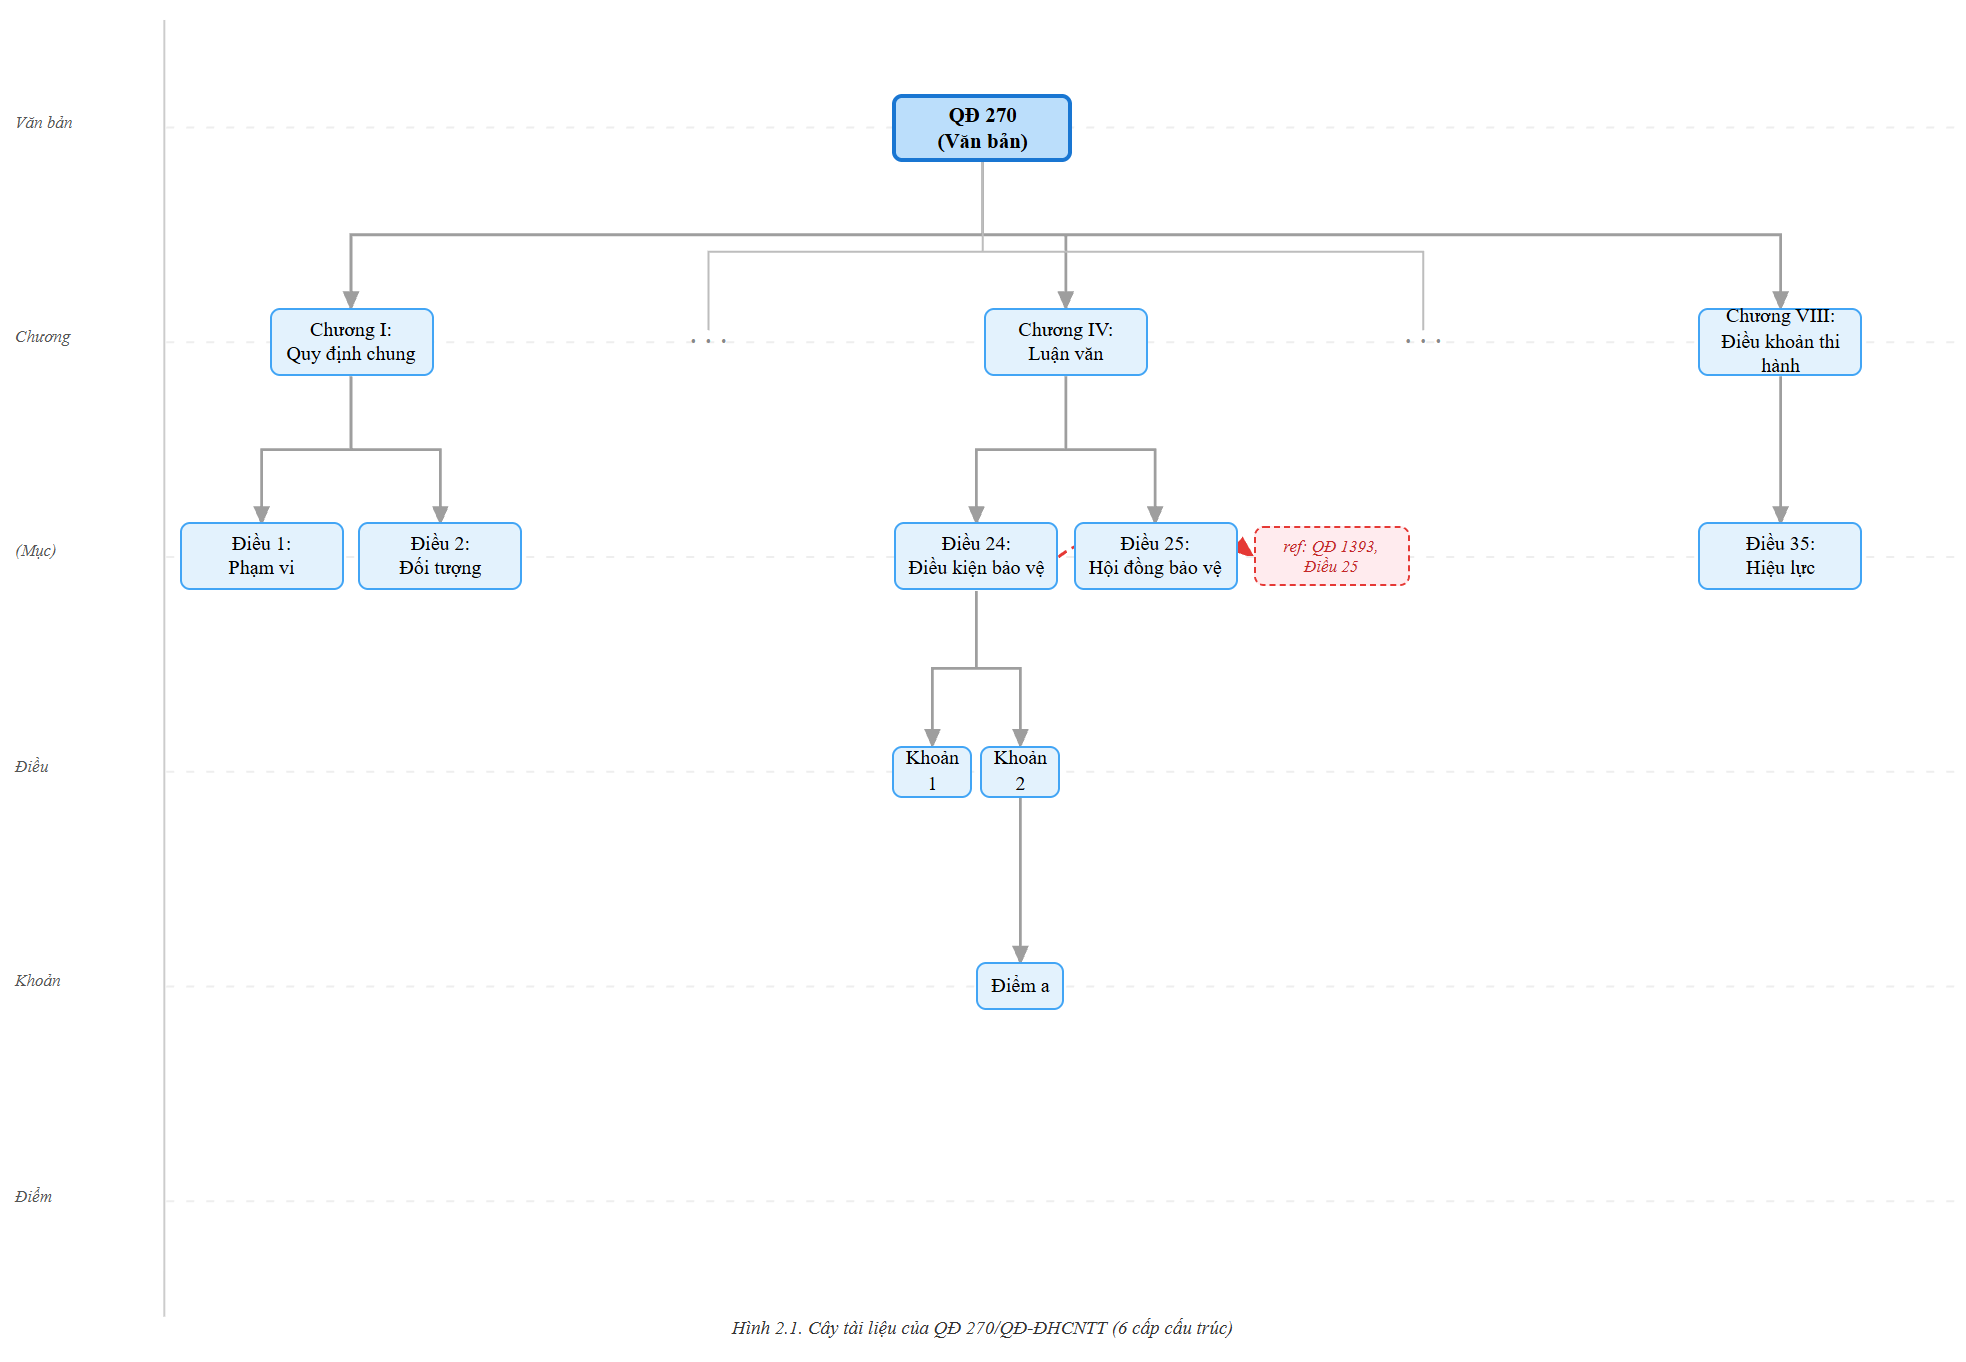
\includegraphics[width=0.95\textwidth]{graphics/figure2-1-document-tree.png}
    \caption{Cấu trúc Document Tree của QĐ~270/QĐ-ĐHCNTT theo cấu trúc phân cấp
    6 cấp: Văn bản $\rightarrow$ Chương $\rightarrow$ Mục $\rightarrow$ Điều
    $\rightarrow$ Khoản $\rightarrow$ Điểm (cấp Mục không áp dụng cho văn bản
    này). Mũi tên nét đứt đỏ thể hiện các tham chiếu chéo giữa các điều khoản
    và giữa các văn bản.}
    \label{fig:document_tree}
\end{figure}

% ------------------------------------------------------------
\subsection{Các quy chế trong phạm vi nghiên cứu}
\label{subsec:cacquiche}

Luận văn sử dụng 5 quy chế đào tạo được liệt kê trong Bảng~\ref{tab:quyche_list},
bao gồm tổng cộng 28 chương và 109 điều. Dưới đây trình bày chi tiết phạm vi,
nội dung chính, và vai trò của từng quy chế trong hệ thống.

\begin{table}[htbp]
    \centering
    \caption{Danh sách các quy chế đào tạo trong phạm vi nghiên cứu}
    \label{tab:quyche_list}
    \begin{tabular}{cp{5.5cm}ccc}
        \toprule
        \textbf{STT} & \textbf{Tên quy chế} & \textbf{Số QĐ} & \textbf{Số chương} & \textbf{Số điều} \\
        \midrule
        1 & Quy chế ĐT trình độ ThS của UIT
          & 270/QĐ-ĐHCNTT & 8 & 35 \\
        2 & Quy chế ĐT trình độ ThS của ĐHQG-HCM (khóa 2021)
          & 160/QĐ-ĐHQG & 7 & 28 \\
        3 & Quy chế ĐT trình độ ThS của ĐHQG-HCM (khóa 2022+)
          & 1393/QĐ-ĐHQG & 8 & 32 \\
        4 & Quy chế sửa đổi bổ sung về GVHD
          & 218/QĐ-ĐHQG & 2 & 6 \\
        5 & Quy định liêm chính học thuật
          & 851/QĐ-ĐHCNTT & 3 & 8 \\
        \midrule
        \multicolumn{3}{r}{\textbf{Tổng cộng}} & \textbf{28} & \textbf{109} \\
        \bottomrule
    \end{tabular}
\end{table}

\subsubsection*{QĐ~270/QĐ-ĐHCNTT -- Quy chế đào tạo trình độ thạc sĩ của UIT}

QĐ~270 được ban hành ngày 25/04/2022, là quy chế đào tạo trình độ thạc sĩ chính
của Trường Đại học Công nghệ Thông tin, gồm 8 chương và 35 điều. Đây là văn bản
được học viên cao học UIT tham chiếu nhiều nhất, quy định toàn bộ quy trình từ
tuyển sinh đến tốt nghiệp.

\begin{sloppypar}
\begin{itemize}
  \item \textbf{Chương I} (Điều 1--4): Quy định chung -- phạm vi áp dụng, đối
        tượng, mục tiêu đào tạo, hình thức đào tạo (tập trung, không tập trung).
  \item \textbf{Chương II} (Điều 5--7): Tuyển sinh -- điều kiện dự tuyển, hồ sơ
        dự tuyển, hình thức xét tuyển.
  \item \textbf{Chương III} (Điều 8--12): Chương trình đào tạo -- khung chương
        trình (60 tín chỉ cho định hướng nghiên cứu, 45 tín chỉ cho ứng dụng),
        các khối kiến thức, đăng ký môn học.
  \item \textbf{Chương IV} (Điều 13--17): Tổ chức đào tạo -- thời gian đào tạo
        (1,5--4 năm), nghỉ phép, chuyển ngành, bảo lưu kết quả.
  \item \textbf{Chương V} (Điều 18--20): Đánh giá kết quả -- thang điểm 0--10
        (quy đổi A/\allowbreak B+/\allowbreak B/\allowbreak C+/\allowbreak
        C/\allowbreak D+/\allowbreak D/\allowbreak F), cảnh báo học vụ, buộc thôi học.
  \item \textbf{Chương VI} (Điều 21--28): Luận văn thạc sĩ -- đề cương, giáo
        viên hướng dẫn, hội đồng xét duyệt đề cương, hội đồng chấm luận văn
        (5 thành viên), điều kiện bảo vệ, quy trình bảo vệ và chỉnh sửa sau
        bảo vệ.
  \item \textbf{Chương VII} (Điều 29--32): Tốt nghiệp -- điều kiện xét tốt
        nghiệp (GPA~$\geq 5{,}5$, luận văn đạt, ngoại ngữ đạt), công nhận tốt
        nghiệp, cấp bằng.
  \item \textbf{Chương VIII} (Điều 33--35): Điều khoản thi hành -- hiệu lực,
        trách nhiệm thi hành, xử lý chuyển tiếp.
\end{itemize}
\end{sloppypar}

\subsubsection*{QĐ~160/QĐ-ĐHQG -- Quy chế khung ĐHQG-HCM (khóa 2021)}

QĐ~160 được ban hành ngày 24/03/2017, là quy chế khung của ĐHQG-HCM áp dụng cho
các khóa đào tạo trước 2022, gồm 7 chương và 28 điều. Quy chế này đặt ra các
nguyên tắc chung mà các trường thành viên phải tuân thủ khi xây dựng quy chế cấp
trường:

\begin{itemize}
  \item Thời gian đào tạo: tối đa 3 năm (ngắn hơn QĐ~1393).
  \item Yêu cầu ngoại ngữ: đạt trình độ B1 theo Khung tham chiếu châu Âu (CEFR)
        hoặc tương đương (TOEIC $\geq$ 450, IELTS $\geq$ 4,0).
  \item Số tín chỉ tối thiểu: 46 tín chỉ cho ThS nghiên cứu, 60 tín chỉ cho ThS
        ứng dụng.
  \item Chưa có quy định về bài báo khoa học bắt buộc.
\end{itemize}

\subsubsection*{QĐ~1393/QĐ-ĐHQG -- Quy chế mới ĐHQG-HCM (khóa 2022+)}

QĐ~1393 được ban hành ngày 03/11/2021, thay thế QĐ~160, áp dụng cho các khóa từ
2022 trở đi, gồm 8 chương và 32 điều. Quy chế mới có nhiều thay đổi quan trọng so
với quy chế cũ. Bảng~\ref{tab:qd160_vs_qd1393} so sánh chi tiết các điểm khác biệt
chính giữa hai phiên bản.

\begin{table}[htbp]
    \centering
    \caption{So sánh điểm khác biệt chính giữa QĐ~160 và QĐ~1393}
    \label{tab:qd160_vs_qd1393}
    \begin{tabular}{lp{4.5cm}p{4.5cm}}
        \toprule
        \textbf{Tiêu chí} & \textbf{QĐ~160 (2017)} & \textbf{QĐ~1393 (2021)} \\
        \midrule
        Thời gian ĐT tối đa & 3 năm & 4 năm \\
        Ngoại ngữ đầu ra & B1 CEFR & B1 CEFR (giữ nguyên) \\
        Bài báo khoa học & Không bắt buộc & Khuyến khích (tùy ngành) \\
        Số tín chỉ ThS NC & $\geq$ 46 & $\geq$ 60 \\
        Định hướng ĐT & NC và ứng dụng & NC, ứng dụng, và kết hợp \\
        Điều khoản GVHD & Cơ bản & Chi tiết hơn (bổ sung bởi QĐ~218) \\
        Luận văn & 15--20 tín chỉ & 15--20 tín chỉ (giữ nguyên) \\
        Chuyển tiếp & -- & HV khóa cũ áp dụng QĐ~160 \\
        \bottomrule
    \end{tabular}
\end{table}

Điểm đáng chú ý là điều khoản chuyển tiếp (Điều 32 QĐ~1393): học viên nhập học
trước năm 2022 tiếp tục áp dụng QĐ~160, tạo ra tình huống hai quy chế cùng hiệu
lực trong giai đoạn chuyển tiếp. Đây là một nguồn câu hỏi phổ biến từ học viên
(``Tôi khóa 2021 thì áp dụng quy chế nào?'') và đặt ra yêu cầu cho hệ thống phải
truy xuất đúng văn bản theo khóa học của người dùng.

\subsubsection*{QĐ~218/QĐ-ĐHQG -- Sửa đổi bổ sung quy định GVHD}

QĐ~218 được ban hành ngày 15/03/2024, sửa đổi và bổ sung một số điều về quy định
giáo viên hướng dẫn trong quy chế đào tạo của ĐHQG-HCM, gồm 2 chương và 6 điều.
Văn bản này quy định chi tiết:

\begin{itemize}
  \item Tiêu chuẩn GVHD: phải có học vị tiến sĩ, có công bố khoa học quốc tế trong
        5 năm gần nhất (ít nhất 1 bài ISI/Scopus).
  \item Số lượng hướng dẫn tối đa: mỗi GVHD hướng dẫn không quá 5 học viên ThS và
        3 NCS cùng lúc (Điều 4).
  \item Trách nhiệm GVHD: theo dõi tiến độ, đánh giá định kỳ, ký xác nhận đề cương
        và luận văn.
  \item Đồng hướng dẫn: cho phép tối đa 2 người đồng hướng dẫn, ít nhất 1 người
        đáp ứng tiêu chuẩn chính.
\end{itemize}

QĐ~218 có mối quan hệ ``sửa đổi bổ sung'' (amend) với QĐ~1393: các điều khoản về
GVHD trong QĐ~1393 được thay thế bởi nội dung tương ứng trong QĐ~218.

\subsubsection*{QĐ~851/QĐ-ĐHCNTT -- Quy định liêm chính học thuật}

QĐ~851 được ban hành ngày 14/08/2024, là quy định về liêm chính học thuật áp dụng
cho học viên cao học UIT, gồm 3 chương và 8 điều:

\begin{itemize}
  \item \textbf{Chương I} (Điều 1--3): Quy định chung -- phạm vi áp dụng, định nghĩa
        đạo văn (plagiarism: sử dụng ý tưởng, dữ liệu, văn bản của người khác mà
        không trích dẫn nguồn), các hình thức vi phạm (tự đạo văn, đạo văn từ nguồn
        khác, gian lận dữ liệu, thuê viết).
  \item \textbf{Chương II} (Điều 4--6): Phát hiện và xử lý -- quy trình phát hiện
        (kiểm tra Turnitin với ngưỡng trùng lặp $\leq 30\%$), hội đồng xác minh,
        các mức xử lý kỷ luật (cảnh cáo, hủy kết quả môn học, đình chỉ học tập, buộc
        thôi học).
  \item \textbf{Chương III} (Điều 7--8): Điều khoản thi hành -- trách nhiệm của GVHD,
        khoa, và phòng đào tạo trong việc giám sát liêm chính.
\end{itemize}

% ============================================================
\section{Các công trình liên quan}
\label{sec:cong-trinh-lien-quan}

Bài toán thu thập, biểu diễn, và truy xuất kiến thức pháp lý là một lĩnh vực nghiên
cứu có lịch sử lâu dài trong trí tuệ nhân tạo và luật học tính toán (computational
law). Phần này trình bày năm hướng nghiên cứu chính liên quan đến luận văn: ontology
pháp lý, mô hình ngôn ngữ cho văn bản pháp lý, truy xuất tăng cường sinh
(Retrieval-Augmented Generation), truy xuất dựa trên đồ thị tri thức, và hỏi đáp
pháp lý tự động.

% ------------------------------------------------------------
\subsection{Ontology và biểu diễn tri thức pháp lý}
\label{subsec:ontology-phap-ly}

Sartor và cộng sự \cite{sartor2011legalonto} trình bày một tuyển tập các phương pháp
xây dựng ontology pháp lý, phân biệt ba tầng: \textit{ontology trên} (upper ontology)
định nghĩa các khái niệm trừu tượng như quy tắc (norm), chủ thể (agent), hành vi
(action); \textit{ontology miền} (domain ontology) đặc tả cho từng lĩnh vực pháp
luật cụ thể; và \textit{ontology ứng dụng} (application ontology) phục vụ tác vụ
riêng biệt. Các tác giả nhấn mạnh rằng ontology pháp lý là nền tảng thiết yếu cho
việc xử lý, truy xuất, và suy luận tự động trên thông tin pháp lý trong bối cảnh
Semantic Web. Mô hình ba tầng này được xác nhận là tối ưu cho việc biểu diễn tri
thức pháp lý trong các bối cảnh khác nhau, từ suy luận lôgic đến truy xuất tài liệu.
Luận văn áp dụng mô hình phân tầng này, trong đó ontology miền cho quy chế đào tạo
được tự động sinh bởi LLM (14 loại thực thể) kết hợp tinh chỉnh thủ công.

Nguyen T. và cộng sự \cite{nguyen2022legalonto} đề xuất Legal-Onto, mô hình hai lớp
cho biểu diễn tri thức văn bản pháp luật: lớp ontology định nghĩa các khái niệm
và quan hệ trong văn bản pháp luật, còn lớp Knowledge Graph hiện thực hóa
ontology phục vụ truy xuất thông minh. Mô hình được thiết kế cho văn bản pháp luật
Việt Nam, tập trung vào cấu trúc phân cấp (chương, mục, điều, khoản) và các quan
hệ giữa các điều khoản. Cách tiếp cận hai lớp này cho phép tách biệt rõ ràng giữa
định nghĩa khái niệm (conceptual layer) và triển khai kỹ thuật (implementation
layer), tạo điều kiện cho việc tái sử dụng ontology qua nhiều ứng dụng khác nhau.
Luận văn kế thừa ý tưởng tích hợp ontology--Knowledge Graph từ Legal-Onto, nhưng
mở rộng bằng việc bổ sung quan hệ ngữ nghĩa (synonym, related, prerequisite) bên
cạnh quan hệ cấu trúc.

Do N.\,V. và cộng sự \cite{do2018rela} đề xuất Rela-model, khung biểu diễn tri thức dựa
trên ontology cho hệ thống chuyên gia, bao gồm ba thành phần: khái niệm (concept),
quan hệ (relation), và quy tắc (rule). Mô hình sử dụng ngôn ngữ đặc tả hình thức
để mô tả cấu trúc tri thức miền, hỗ trợ suy luận dựa trên quy tắc trên dữ liệu
có cấu trúc. Điểm mạnh của Rela-model là khả năng biểu diễn các luật suy luận phức
tạp và các ràng buộc (constraints) trên dữ liệu, điều này đặc biệt hữu ích cho
miền pháp lý nơi các quy tắc và điều kiện là trung tâm. Luận văn tham khảo cách
tiếp cận quan hệ hóa (relation-based) của Rela-model khi thiết kế lược đồ quan hệ
cho Knowledge Graph pháp lý.

Ngo H. và cộng sự \cite{ngo2024ontology} đề xuất phương pháp ontology Knowledge Map
cho việc xây dựng Linked Data cho các ứng dụng pháp lý tiếng Việt. Nghiên cứu này
xử lý kho dữ liệu lớn gồm khoảng 325.000 tài liệu pháp lý, đề xuất Legal-Onto
model kết hợp ontology làm lớp khái niệm (conceptual layer) và Knowledge Graph làm
lớp triển khai (implementation layer). Một đóng góp quan trọng của công trình này là
cách tiếp cận hệ thống để trích xuất ontology từ một khối lượng lớn tài liệu pháp
lý không có cấu trúc, sử dụng kỹ thuật xử lý ngôn ngữ tự nhiên để tự động nhận
diện khái niệm và quan hệ. Phương pháp này trực tiếp hỗ trợ bài toán của luận văn
về việc tự động sinh ontology miền cho quy chế đào tạo từ tài liệu gốc.

Pham V. và cộng sự \cite{pham2024enhancing} đề xuất cách tiếp cận tri thức được tích
hợp (knowledge-infused) cho truy xuất thông tin pháp lý trong lĩnh vực luật lao động
tiếng Việt. Nghiên cứu sử dụng tập dữ liệu gồm 300.000 tài liệu được phân loại
thành 20 loại tài liệu pháp lý và 27 lĩnh vực pháp lý, xây dựng bộ câu hỏi--trả
lời (Q\&A dataset) riêng cho lĩnh vực luật lao động và tích hợp ontology pháp lý
vào quy trình truy xuất. Kết quả cho thấy việc tích hợp tri thức ontology cải thiện
đáng kể hiệu suất truy xuất so với các phương pháp không sử dụng tri thức, chứng
minh hiệu quả của việc kết hợp Knowledge Graph và ontology cho truy xuất tài liệu
pháp lý tiếng Việt -- một kết quả mà luận văn tận dụng cho miền quy chế đào tạo.

Pham V. và cộng sự \cite{pham2026ontology} đề xuất phương pháp Knowledge Graph dựa
trên ontology cho hệ thống truy xuất thông tin pháp lý tự động, nhấn mạnh tích hợp
sâu giữa ontology làm lớp khái niệm và Knowledge Graph làm lớp triển khai. Phương
pháp được thiết kế để xử lý các vấn đề chính trong miền pháp lý: tự động trích xuất
thông tin từ tài liệu không có cấu trúc, suy luận trên các quan hệ phức tạp giữa
các khái niệm pháp lý, và trả lời các truy vấn yêu cầu suy luận đa bước. Công
trình chứng minh rằng Knowledge Graph kết hợp với ontology pháp lý cải thiện độ
chính xác truy xuất so với các phương pháp truyền thống, cung cấp nền tảng lý thuyết
cho thiết kế Tầng~3 của luận văn nơi Knowledge Graph kết hợp suy luận đồ thị được
sử dụng để mở rộng kết quả truy xuất.

% ------------------------------------------------------------
\subsection{Mô hình ngôn ngữ và NLP cho văn bản pháp lý}
\label{subsec:nlp-phap-ly}

Devlin và cộng sự \cite{devlin2019bert} giới thiệu BERT (Bidirectional Encoder
Representations from Transformers), kiến trúc mô hình ngôn ngữ tiền huấn luyện hai
chiều đạt kết quả vượt trội trên 11 tác vụ NLP. BERT trở thành nền tảng cho hầu
hết các mô hình ngôn ngữ chuyên biệt miền sau này, bao gồm cả miền pháp lý.

Chalkidis và cộng sự \cite{chalkidis2020legalbert} giới thiệu LEGAL-BERT, mô hình
ngôn ngữ được tiền huấn luyện trên kho văn bản pháp lý tiếng Anh (bao gồm luật
của EU, UK, và Mỹ). Thông qua tìm kiếm siêu tham số mở rộng, nghiên cứu chứng
minh rằng các hướng dẫn tinh chỉnh (fine-tuning) từ NLP đa dụng không tổng quát
hóa tốt cho miền pháp lý -- mô hình chuyên biệt miền vượt trội so với mô hình đa
ngôn ngữ (XLM-R) và BERT tổng quát trên các tác vụ phân loại văn bản pháp luật
và rà soát hợp đồng.

Zhong và cộng sự \cite{zhong2020nlplaw} tổng hợp hệ thống các ứng dụng NLP trong
lĩnh vực pháp luật, phân loại thành năm nhóm tác vụ chính: phân loại văn bản pháp
lý, nhận dạng thực thể, trích xuất thông tin, tóm tắt văn bản, và hỏi đáp pháp lý.
Nghiên cứu chỉ ra rằng miền pháp lý đặt ra các thách thức đặc thù: thuật ngữ
chuyên ngành, nhạy cảm ngữ cảnh cao, và sự thay đổi thường xuyên của quy định.

\begin{sloppypar}
Đối với tiếng Việt, Nguyen D.\,Q. và Nguyen A.\,T. \cite{nguyen2020phobert} phát triển PhoBERT,
mô hình ngôn ngữ tiền huấn luyện đơn ngữ cho tiếng Việt gồm hai phiên bản
(PhoBERT\textsubscript{base} và PhoBERT\textsubscript{large}), được huấn luyện trên
kho ngữ liệu tiếng Việt lớn. PhoBERT vượt trội so với mô hình đa ngôn ngữ XLM-R
trên các tác vụ gán nhãn từ loại, phân tích cú pháp phụ thuộc, nhận dạng thực thể,
và suy luận ngôn ngữ tự nhiên -- khẳng định rằng mô hình đơn ngữ là thiết yếu cho
các ngôn ngữ có hình thái phong phú. Vu T. và cộng sự \cite{vu2018vncore} phát triển
VnCoreNLP, bộ công cụ NLP mã nguồn mở cho tiếng Việt, tích hợp phân đoạn từ
(word segmentation), gán nhãn từ loại (POS tagging), nhận dạng thực thể (NER), và
phân tích cú pháp phụ thuộc (dependency parsing), đạt kết quả tiên tiến nhất
(state-of-the-art) trên các tập dữ liệu chuẩn tiếng Việt tại thời điểm công bố.
\end{sloppypar}

Tuy nhiên, các công cụ NLP tiếng Việt nêu trên chưa được tối ưu cho văn bản pháp
lý, đặc biệt trong việc nhận diện viết tắt chuyên ngành (ThS, NCS, GVHD), thuật
ngữ pháp lý, và cấu trúc tham chiếu (``theo Điều X Khoản Y''). Luận văn bổ sung
bước tiền xử lý chuyên biệt gồm mở rộng viết tắt (49 mục), ánh xạ đồng nghĩa
(18 cặp), và trích xuất thực thể giống (seed entity extraction) trước khi truy xuất.

Reimers và Gurevych \cite{reimers2019sbert} đề xuất Sentence-BERT (SBERT), phương
pháp tính embedding cấp câu dựa trên mạng Siamese BERT. Mặc dù BERT gốc đạt hiệu
suất tốt nhất trên các tác vụ so khớp cặp câu (semantic textual similarity), mô
hình này yêu cầu cả hai câu phải được đưa vào mạng cùng lúc, dẫn đến chi phí tính
toán khổng lồ: việc tìm cặp câu giống nhất từ 10.000 câu yêu cầu khoảng 50 triệu
phép suy luận (~65 giờ). Sentence-BERT sử dụng cấu trúc mạng Siamese và Triplet để
tính embedding câu một cách độc lập, cho phép so sánh bằng cosine-similarity trên
các vector embedding, giảm thời gian tìm kiếm xuống còn khoảng 5 giây trong khi vẫn
duy trì độ chính xác tương đương. Sentence-BERT đã trở thành phương pháp chuẩn (de
facto standard) cho tính toán embedding câu trong hệ thống truy xuất vector hiện đại.
Luận văn sử dụng Sentence-BERT tại Tầng~2 của pipeline truy xuất để tính embedding
cho các điều khoản và câu hỏi người dùng, cho phép truy xuất nhanh chóng các điều
khoản liên quan dựa trên tương đồng ngữ nghĩa.

% ------------------------------------------------------------
\subsection{Truy xuất tăng cường sinh (RAG)}
\label{subsec:rag}

Lewis và cộng sự \cite{lewis2020rag} đề xuất kiến trúc RAG (Retrieval-Augmented
Generation), kết hợp bộ truy xuất (retriever) dựa trên bộ mã hóa kép (dual-encoder)
với bộ sinh (generator) seq2seq tiền huấn luyện, huấn luyện đầu-cuối
(end-to-end) thông qua tìm kiếm tích nội tối đa (MIPS). RAG vượt trội so với mô
hình seq2seq thuần trên các tác vụ đòi hỏi kiến thức (knowledge-intensive) như hỏi
đáp miền mở (open-domain QA), xác minh sự kiện (fact verification), nhờ việc neo
(grounding) quá trình sinh vào các tài liệu nguồn cụ thể. Sự kết hợp giữa bộ truy
xuất và bộ sinh cho phép mô hình tiếp cận thông tin cập nhật từ kho tài liệu bên
ngoài mà không cần huấn luyện lại toàn bộ các thông số mô hình. Kiến trúc RAG trở
thành nền tảng cho hệ thống hỏi đáp có căn cứ -- đặc biệt quan trọng trong miền
pháp lý nơi câu trả lời phải trích dẫn được nguồn.

Karpukhin và cộng sự \cite{karpukhin2020dpr} giới thiệu DPR (Dense Passage
Retrieval), sử dụng bộ mã hóa kép huấn luyện với hàm mất mát tương phản
(contrastive loss) trên các cặp câu hỏi--đoạn văn. DPR vượt trội BM25 từ
9--19\% độ chính xác truy xuất cấp đoạn văn, chứng minh rằng biểu diễn dày đặc
(dense representation) nắm bắt tương đồng ngữ nghĩa tốt hơn phương pháp thưa
(sparse). Phương pháp dual-encoder của DPR cho phép mã hóa độc lập câu hỏi và
tài liệu, tạo điều kiện thuận lợi cho truy xuất nhanh bằng tính toán vector tương
đồng. Luận văn sử dụng cách tiếp cận embedding dày đặc tương tự tại Tầng~2
của pipeline truy xuất.

Fan và cộng sự \cite{fan2024ragsurvey} khảo sát hệ thống các kiến trúc RAG kết
hợp LLM, phân loại theo ba chiều: kiến trúc (retriever-reader, retriever-generator),
chiến lược huấn luyện (huấn luyện retriever, generator, hoặc đồng thời), và ứng
dụng (tăng tính chính xác, cập nhật kiến thức, tác vụ chuyên biệt miền). Nghiên
cứu xác nhận rằng RAG chuyên biệt miền vượt trội so với RAG đa dụng, với các hệ
thống miền cụ thể đạt được độ chính xác cao hơn 10--20\% so với mô hình đa dụng
trên các tác vụ hẹp, củng cố lựa chọn của luận văn về việc thiết kế pipeline truy
xuất riêng cho miền quy chế đào tạo.

Gao và cộng sự \cite{gao2023hyde} đề xuất HyDE (Hypothetical Document Expansion),
cách tiếp cận zero-shot cho truy xuất dày đặc không cần nhãn liên quan. Thay vì
truy xuất trực tiếp từ truy vấn người dùng, HyDE sử dụng LLM để tạo ra tài liệu
giả thuyết (hypothetical document) có thể trả lời truy vấn, sau đó mã hóa tài liệu
này bằng encoder không giám sát và sử dụng dense bottleneck để lọc bỏ ảo giác, chỉ
giữ lại các tài liệu thực tế có vector tương đồng cao. HyDE đạt kết quả tương đương
hoặc vượt trội DPR trên các bộ dữ liệu QA mở và xác minh sự kiện, đồng thời mở
rộng được sang các ngôn ngữ không phải tiếng Anh.

Sarthi và cộng sự \cite{sarthi2024raptor} đề xuất RAPTOR (Recursive Abstractive
Processing for Tree-Organized Retrieval), giải quyết hạn chế của RAG truyền thống
khi xử lý các tài liệu dài. RAPTOR xây dựng cây phân cấp bằng cách đệ quy nhúng,
phân cụm, và tóm tắt các khối văn bản từ dưới lên trên, tạo ra các mức tóm tắt
khác nhau từ chi tiết cụ thể đến tổng quát hóa toàn bộ tài liệu. Tại thời điểm
suy luận, hệ thống truy xuất từ các mức cây khác nhau phù hợp với yêu cầu câu hỏi,
tích hợp thông tin ở nhiều mức độ trừu tượng. Trên bộ dữ liệu QuALITY yêu cầu suy
luận phức tạp đa bước, RAPTOR cải thiện kết quả 20\% tuyệt đối khi kết hợp với
GPT-4. RAPTOR được sử dụng làm baseline đánh giá trong Chương~\ref{chap:chapter4};
so sánh cho thấy pipeline 3 tầng của luận văn vượt trội RAPTOR nhờ kết hợp duyệt
cây theo hướng dẫn LLM, truy xuất ngữ nghĩa hai cấp, và mở rộng qua Knowledge
Graph thay vì chỉ sử dụng cây phân cấp tóm tắt.

Asai và cộng sự \cite{asai2024selfrag} đề xuất Self-RAG, khung cho phép mô hình
ngôn ngữ tự động quyết định khi nào cần truy xuất và đánh giá chất lượng tài liệu
được truy xuất. Khác với RAG truyền thống luôn truy xuất một số lượng cố định tài
liệu, Self-RAG huấn luyện mô hình truy xuất linh hoạt: có thể truy xuất nhiều lần
trong quá trình sinh hoặc bỏ qua truy xuất hoàn toàn, sử dụng các reflection tokens
để đánh giá cả tài liệu truy xuất lẫn nội dung sinh ra. Self-RAG (7B và 13B tham
số) vượt trội ChatGPT và Llama2-chat trên các tác vụ hỏi đáp miền mở, suy luận,
và xác minh sự kiện, đồng thời cải thiện tính xác thực (factuality) và độ chính xác
trích dẫn. Cách tiếp cận phản xạ (self-reflection) của Self-RAG có ảnh hưởng đến
thiết kế Tầng~1 của luận văn, nơi LLM được sử dụng để duyệt cây quy định một cách
thông minh.

Zhang và Tang \cite{zhang2025pageindex} giới thiệu PageIndex, khung RAG không sử
dụng vector database (vectorless RAG) dựa trên suy luận LLM. Thay vì dựa vào vector
similarity search, PageIndex xây dựng chỉ mục cấu trúc cây từ tài liệu và cho phép
LLM thực hiện suy luận trên cấu trúc đó, mô phỏng cách chuyên gia con người điều
hướng tài liệu phức tạp. PageIndex không yêu cầu chia nhỏ tài liệu (chunking) mà
tổ chức chúng vào các phần tự nhiên, cải thiện khả năng truy vết (explainability).
Trên bộ dữ liệu tài chính FinanceBench, PageIndex đạt 98,7\% độ chính xác. PageIndex
cũng được sử dụng làm baseline trong Chương~\ref{chap:chapter4}; so sánh cho thấy
pipeline 3 tầng của luận văn vượt trội PageIndex khoảng 7--13 điểm phần trăm trên
Hit@10, nhờ kết hợp truy xuất đa phương pháp: duyệt cây, embedding dày đặc, và mở
rộng Knowledge Graph.

% ------------------------------------------------------------
\subsection{Truy xuất dựa trên đồ thị tri thức}
\label{subsec:graph-rag}

Edge và cộng sự \cite{edge2024graphrag} đề xuất GraphRAG, phương pháp tiên tiến
giải quyết hạn chế của RAG truyền thống trên các câu hỏi đòi hỏi tổng hợp toàn
cục (global sensemaking queries) như ``các chủ đề chính là gì?''. GraphRAG sử dụng
LLM để trích xuất đồ thị tri thức thực thể từ tài liệu, sau đó sinh trước các bản
tóm tắt cộng đồng (community summaries) cho từng cụm thực thể dựa trên cấu trúc
phân cấp, rồi tổng hợp câu trả lời từ các bản tóm tắt này thay vì trực tiếp từ
văn bản. Phương pháp cải thiện đáng kể tính toàn diện và đa dạng của câu trả lời
so với RAG truyền thống, đồng thời cho phép mở rộng đến tập dữ liệu lớn (1 triệu
token) nhờ cấu trúc cộng đồng phân cấp. GraphRAG đã được triển khai trong các ứng
dụng quản lý tri thức tại Microsoft, chứng minh khả năng ứng dụng thực tế.

Guo và cộng sự \cite{guo2025lightrag} đề xuất LightRAG, khung truy xuất tối ưu hơn
bằng cách tích hợp cấu trúc đồ thị trực tiếp vào quá trình đánh chỉ mục (indexing).
LightRAG sử dụng hệ thống truy xuất hai cấp giúp khám phá thông tin ở cả mức thấp
(low-level) cho các thực thể cụ thể và quan hệ chi tiết, và mức cao (high-level)
cho các chủ đề tổng quát và cộng đồng thực thể, đồng thời tích hợp cấu trúc đồ thị
với biểu diễn vector để truy xuất hiệu quả các thực thể liên quan và mối quan hệ
giữa chúng. LightRAG vượt trội so với NaiveRAG, RQ-RAG, HyDE, và chính GraphRAG
trên bốn miền ứng dụng, bao gồm rõ ràng \textbf{miền pháp lý}. Cơ chế truy xuất
hai cấp độ của LightRAG có ảnh hưởng trực tiếp đến thiết kế Tầng~2 của luận văn
(xem Chương~\ref{chap:thiet-ke-giai-thuat}), nơi truy xuất cấp thực thể
(low-level) và cấp chủ đề (high-level) được tích hợp.

\begin{sloppypar}
Mavromatis và Karypis \cite{mavromatis2024gnnrag} đề xuất GNN-RAG, sử dụng mạng
nơ-ron đồ thị (Graph Neural Network) để trích xuất các đường lý luận
(reasoning paths) có độ dài ngắn nhất trên đồ thị tri thức, kết nối trực tiếp từ
thực thể được đề cập trong câu hỏi đến các ứng viên câu trả lời. Sau khi trích
xuất, các đường lý luận được chuyển đổi thành dạng văn bản tự nhiên để LLM có thể
suy luận dựa trên bối cảnh. GNN-RAG đạt kết quả tiên tiến trên các tập dữ liệu
KGQA công khai WebQSP và CWQ, vượt phương pháp truy xuất bằng LLM từ
8,9--15,5\% F1 trên các câu hỏi đa bước (multi-hop), đồng thời chỉ sử dụng khoảng
1/9 số token so với phương pháp ngữ cảnh dài (long-context). Ý tưởng trích xuất
đường lý luận trên đồ thị tương đồng với cơ chế mở rộng KG tại Tầng~3 của luận
văn, nơi PPR (Personalized PageRank) được dùng để tìm các thực thể liên quan qua
suy luận đa bước.
\end{sloppypar}

Cấu trúc các phương pháp truy xuất dựa trên đồ thị xây dựng trên nền tảng lý
thuyết của các thuật toán xếp hạng trên đồ thị, đặc biệt là các biến thể của
PageRank. Haveliwala \cite{haveliwala2002ppr} giới thiệu Topic-Sensitive PageRank,
phương pháp tính toán nhiều vector PageRank độc lập, mỗi vector được thiên lệch
theo một chủ đề cụ thể, cho phép xếp hạng các nút đồ thị dựa trên tầm quan trọng
so với chủ đề đó. Jeh và Widom \cite{jeh2003ppr} mở rộng công trình này bằng
phương pháp tính toán vector PageRank cá nhân hóa theo tập hợp các trang được người
dùng quan tâm, giải quyết bài toán tính toán hiệu quả mà không cần thực hiện lặp
lại đầy đủ cho từng cá nhân hóa. Gleich \cite{gleich2015pagerank} thực hiện khảo
sát toàn diện về ứng dụng PageRank ngoài lĩnh vực tìm kiếm web, chứng minh rằng
toán học PageRank là tổng quát và áp dụng được trên bất kỳ đồ thị hoặc mạng nào.
Các công trình nền tảng này cung cấp cơ sở lý thuyết cho việc áp dụng PPR trong
cơ chế mở rộng tri thức tại Tầng~3 của luận văn.

% ------------------------------------------------------------
\subsection{Hỏi đáp pháp lý tự động}
\label{subsec:hoi-dap-phap-ly}

Lai và cộng sự \cite{lai2024llmlaw} thực hiện khảo sát toàn diện và hệ thống về ứng
dụng của các mô hình ngôn ngữ lớn trong lĩnh vực pháp luật, với tiêu chí đánh giá
11 bộ benchmark năng lực pháp lý (CaseLaw, DISC-Law-Eval, KBL, LAiW, LawBench, LBOX
OPEN, LegalBench, LexEval, LexGLUE, SimuCourt, SMILED) và 4 bộ benchmark tác vụ
chuyên biệt. Nghiên cứu chỉ ra rằng LLM cho thấy tiềm năng lớn trong ba lĩnh vực
chính: tư vấn pháp lý, hỗ trợ quyết định cho thẩm phán, và phân tích tài liệu pháp
luật. Tuy nhiên, các mô hình đối mặt ba thách thức: dữ liệu huấn luyện pháp lý
còn hạn chế so với dữ liệu chung; vấn đề đạo đức và trách nhiệm pháp lý khi sử
dụng AI trong quyết định pháp lý; và ảo giác (hallucination) -- hiện tượng mô
hình phát sinh thông tin sai khi thiếu ngữ cảnh chính xác. Kết luận này củng cố lựa
chọn kiến trúc RAG của luận văn: LLM cần bước truy xuất rõ ràng từ tài liệu gốc để
đảm bảo câu trả lời có căn cứ pháp lý và giảm thiểu rủi ro ảo giác.

Ngo Q.\,H. và cộng sự \cite{ngo2021aimelaw} phát triển AimeLaw, hệ thống hỏi đáp pháp lý
tiếng Việt tham gia cuộc thi Automated Legal Question Answering Competition
(ALQAC)~2021. Hệ thống kết hợp ba thành phần chính: truy xuất từ điển (BM25), mô
hình BERT tiền huấn luyện trên tập dữ liệu lớn, và tăng cường dữ liệu nhận biết
miền pháp lý (domain-aware data augmentation) -- kỹ thuật tạo mẫu huấn luyện nhân
tạo dựa trên kiến thức miền. Hệ thống đạt kết quả nổi bật: suy luận văn bản pháp
lý (legal textual entailment) 69,89\% chính xác (giải nhất), truy xuất văn bản pháp
lý 80,61\% F2 (giải nhì), hỏi đáp pháp lý 64,77\% chính xác (giải nhì). Kết quả
cho thấy tích hợp tri thức miền pháp lý cải thiện đáng kể hiệu suất so với mô hình
nơ-ron thuần -- một quan sát phù hợp với cách tiếp cận Knowledge Graph của luận văn.

Nguyen H. và cộng sự \cite{nguyen2024intelligent} phát triển hệ thống tìm kiếm thông
minh cho việc khớp hồ sơ công việc và truy vấn luật lao động Việt Nam. Hệ thống sử
dụng phương pháp dựa trên ontology để giải quyết hai bài toán: khớp kỹ năng
công việc giữa hồ sơ ứng viên và mô tả công việc, đồng thời tìm kiếm các quy định
pháp luật lao động liên quan. Nhóm tác giả xây dựng hai ontology riêng biệt -- một
ontology kỹ năng và một ontology pháp luật lao động -- tích hợp vào cùng một cơ sở
tri thức. Hệ thống đạt kết quả tốt nhất trên các truy vấn về bảo hiểm thất nghiệp
(độ chính xác trên 70\%), chứng minh hiệu quả của phương pháp biểu diễn tri thức
dựa trên ontology cho các lĩnh vực pháp lý Việt Nam.

Ho X. và cộng sự \cite{ho2020constructing} trình bày phương pháp xây dựng tập dữ liệu
hỏi đáp đa bước (multi-hop QA dataset) gọi là 2WikiMultiHopQA, kết hợp dữ liệu có
cấu trúc (từ Wikidata) và dữ liệu phi cấu trúc (văn bản Wikipedia). Đặc điểm nổi
bật là mỗi câu hỏi đi kèm thông tin bằng chứng (evidence) chứa đường suy luận
(reasoning path) rõ ràng, cho phép đánh giá không chỉ độ chính xác câu trả lời mà
còn chất lượng quá trình suy luận. Phương pháp này đặc biệt liên quan đến luận văn
vì các câu hỏi về quy chế đào tạo thường yêu cầu suy luận đa bước: cần kết hợp
thông tin từ nhiều điều khoản, từ nhiều tầng quy chế (ĐHQG-HCM và UIT), hoặc từ
các quy định liên quan để tạo thành câu trả lời hoàn chỉnh.

\vspace{0.5em}
\noindent\textbf{Tổng hợp và vị trí của luận văn.} Bảng~\ref{tab:related-work-compare}
so sánh các đặc trưng chính của luận văn với các công trình liên quan. Luận văn khác
biệt ở ba điểm: sử dụng kiến trúc truy xuất 3 tầng (duyệt cây + semantic + KG
fusion) thay vì truy xuất đơn tầng; khai thác cấu trúc phân cấp đặc thù của
văn bản quy phạm Việt Nam (6 cấp: văn bản $\rightarrow$ chương $\rightarrow$ mục
$\rightarrow$ điều $\rightarrow$ khoản $\rightarrow$ điểm) thay vì coi tài liệu như
tập hợp phẳng; và kết hợp Knowledge Graph với PPR để mở rộng kết quả truy xuất
qua suy luận đa bước trên đồ thị quan hệ, thay vì chỉ dùng community summaries
như GraphRAG hoặc dual-level retrieval như LightRAG.

\begin{table}[htbp]
    \centering
    \caption{So sánh các công trình liên quan với luận văn}
    \label{tab:related-work-compare}
    \small
    \begin{tabular}{p{2.8cm}cccc}
        \toprule
        \textbf{Công trình} & \textbf{KG} & \textbf{Đa tầng} &
        \textbf{Cấu trúc VB} & \textbf{Tiếng Việt} \\
        \midrule
        RAG \cite{lewis2020rag} & -- & -- & -- & -- \\
        DPR \cite{karpukhin2020dpr} & -- & -- & -- & -- \\
        RAPTOR \cite{sarthi2024raptor} & -- & Cây & $\checkmark$ & -- \\
        Self-RAG \cite{asai2024selfrag} & -- & -- & -- & -- \\
        PageIndex \cite{zhang2025pageindex} & -- & -- & $\checkmark$ & -- \\
        GraphRAG \cite{edge2024graphrag} & $\checkmark$ & -- & -- & -- \\
        LightRAG \cite{guo2025lightrag} & $\checkmark$ & 2 cấp & -- & -- \\
        GNN-RAG \cite{mavromatis2024gnnrag} & $\checkmark$ & -- & -- & -- \\
        AimeLaw \cite{ngo2021aimelaw} & -- & -- & -- & $\checkmark$ \\
        Legal-Onto \cite{nguyen2022legalonto} & $\checkmark$ & -- & $\checkmark$ & $\checkmark$ \\
        \textbf{Luận văn} & $\checkmark$ & 3 tầng & $\checkmark$ & $\checkmark$ \\
        \bottomrule
    \end{tabular}
\end{table}

% ============================================================
\section{Thu thập kiến thức trong văn bản quy chế}
\label{sec:thuthap_kienthuc}

% ------------------------------------------------------------
\subsection{Quy trình thu thập và số hóa}
\label{subsec:quytrinh_thuthap}

Quá trình thu thập kiến thức từ các văn bản quy chế đào tạo được thực hiện qua bốn
bước chính, từ thu thập văn bản gốc đến tạo các biểu diễn tri thức phục vụ truy
xuất.

\textbf{Bước 1: Thu thập văn bản gốc.}
Các quyết định được tải từ website chính thức của UIT
(\texttt{uit.edu.vn/phong-dao-tao}) và ĐHQG-HCM (\texttt{vnuhcm.edu.vn}). Tổng
cộng 5 văn bản với 118 trang PDF, trong đó 4 văn bản ở dạng PDF scan (không có text
layer) và 1 văn bản ở dạng PDF text. Các văn bản PDF scan được số hóa bằng LLM
Vision OCR (Gemini Flash) với độ chính xác cao hơn OCR truyền thống nhờ khả năng
hiểu ngữ cảnh và sửa lỗi tự động. Kết quả OCR được rà soát thủ công để đảm
bảo tính chính xác, đặc biệt với các số hiệu điều khoản và tên riêng.

\textbf{Bước 2: Phân tích cấu trúc.}
Sử dụng bộ phân tích cú pháp (parser) tùy chỉnh với regex nhận diện các dấu hiệu
phân cấp tiếng Việt. Bộ regex bao gồm các mẫu:

\begin{itemize}
  \item Chương: \texttt{Ch\textbackslash ương\textbackslash s+[IVXLC]+} (số La Mã)
        hoặc \texttt{CHƯƠNG\textbackslash s+\textbackslash d+} (số Ả Rập)
  \item Điều: \texttt{Đi\textbackslash ều\textbackslash s+\textbackslash d+}
  \item Khoản: \texttt{\textasciicircum\textbackslash d+\textbackslash .} (số + dấu chấm đầu
        dòng)
  \item Điểm: \texttt{\textasciicircum[a-zđ]\textbackslash )} (chữ cái + ngoặc đóng đầu dòng)
\end{itemize}

Parser xây dựng cây cấu trúc phân cấp bằng thuật toán đẩy--kéo (push--pop) trên
stack: mỗi dấu hiệu mới ở cấp cao hơn đóng tất cả nút con đang mở, tạo nút mới
và đẩy vào stack. Kết quả là một cây có gốc (rooted tree) cho mỗi văn bản, với
metadata (số hiệu, ngày ban hành, cơ quan ban hành) gắn vào nút gốc.

\textbf{Bước 3: Trích xuất tham chiếu chéo.}
Nhận diện các tham chiếu giữa các điều khoản bằng pattern matching trên các chuỗi
trích dẫn. Các mẫu phổ biến bao gồm:

\begin{itemize}
  \item Tham chiếu nội bộ: ``theo quy định tại Điều 5'', ``căn cứ Khoản 1 Điều 24''
  \item Tham chiếu ngoại bộ: ``theo Điều 25 Quy chế đào tạo ĐHQG-HCM''
  \item Tham chiếu thay thế: ``thay thế QĐ~160/QĐ-ĐHQG ngày 24/03/2017''
\end{itemize}

Mỗi tham chiếu được phân loại theo kiểu: THAM\_CHIẾU (dẫn chiếu chung), SỬA\_ĐỔI
(amend), hoặc THAY\_THẾ (replace). Tổng cộng phát hiện 168 tham chiếu chéo trong 5
văn bản, trong đó 134 tham chiếu nội bộ và 34 tham chiếu ngoại bộ.

\textbf{Bước 4: Tạo tóm tắt.}
Sinh tóm tắt cho từng chương và điều bằng LLM (Claude 3.5 Haiku), tạo mô tả gồm
tiêu đề và nhiều từ khóa đặc trưng phục vụ cho bước chọn nhánh trong Tầng~1 của
pipeline truy xuất. Tổng cộng sinh 17 tóm tắt chương và 109 tóm tắt điều. Mỗi tóm
tắt chương bao gồm: phạm vi điều khoản (ví dụ: ``Điều 1--4''), chủ đề chính, và
danh sách 5--10 từ khóa đặc trưng. Mỗi tóm tắt điều bao gồm: tiêu đề điều và 3--5
từ khóa nội dung chính.

Bảng~\ref{tab:thongke_sohoa} tóm tắt kết quả quá trình số hóa và phân tích cấu
trúc.

\begin{table}[htbp]
    \centering
    \caption{Thống kê kết quả số hóa và phân tích cấu trúc}
    \label{tab:thongke_sohoa}
    \begin{tabular}{lr}
        \toprule
        \textbf{Thành phần} & \textbf{Số lượng} \\
        \midrule
        Văn bản quy chế       & 5 \\
        Tổng số trang PDF     & 118 \\
        Chương                & 28 \\
        Điều khoản            & 109 \\
        Khoản                 & $\approx$ 380 \\
        Điểm                  & $\approx$ 520 \\
        Tham chiếu chéo nội bộ & 134 \\
        Tham chiếu chéo ngoại bộ & 34 \\
        Tóm tắt chương        & 17 \\
        Tóm tắt điều          & 109 \\
        \bottomrule
    \end{tabular}
\end{table}

% ------------------------------------------------------------
\subsection{Các khái niệm chính trong quy chế đào tạo}
\label{subsec:khainiemchinh}

Qua phân tích nội dung 5 quy chế, các khái niệm chính (domain concepts) được xác
định và phân loại theo ontology miền. Các khái niệm này đóng vai trò làm thực thể
(entity) trong Knowledge Graph và giúp hệ thống hiểu mối quan hệ ngữ nghĩa giữa
các điều khoản.

\begin{itemize}
    \item \textbf{Chương trình đào tạo}: khung chương trình, môn học bắt buộc, môn
          học tự chọn, số tín chỉ tối thiểu (60 TC cho nghiên cứu, 45 TC cho ứng
          dụng), khối kiến thức cơ sở ngành và chuyên ngành.

    \item \textbf{Tín chỉ và môn học}: định nghĩa tín chỉ (15 tiết lý thuyết hoặc
          30 tiết thực hành), phân loại môn học (bắt buộc, tự chọn, bổ sung), điều
          kiện tiên quyết, quy trình đăng ký và hủy môn học.

    \item \textbf{Đánh giá kết quả học tập}: thang điểm 10 (0--10), thang điểm 4
          (0--4), thang điểm chữ (A, B+, B, C+, C, D+, D, F), bảng quy đổi giữa
          các thang điểm. Ví dụ: 8,5--10 điểm $=$ A $=$ 4,0 điểm hệ 4 $=$ Giỏi.

    \item \textbf{Thời hạn đào tạo}: thời gian chuẩn (1,5--2 năm), thời gian tối
          đa (4 năm theo QĐ~1393, 3 năm theo QĐ~160), quy trình gia hạn (đơn xin
          gia hạn $\to$ khoa xét $\to$ phòng đào tạo phê duyệt), bảo lưu kết quả
          học tập (tối đa 2 năm).

    \item \textbf{Luận văn thạc sĩ}: đề cương luận văn (nộp sau khi hoàn thành
          $\geq$ 70\% tín chỉ), hội đồng xét duyệt đề cương (3 thành viên), giáo
          viên hướng dẫn (tiêu chuẩn, số lượng tối đa), hội đồng bảo vệ luận văn
          (5 thành viên: chủ tịch, thư ký, 2 phản biện, ủy viên), quy trình bảo vệ
          (trình bày 20--30 phút, hỏi đáp 30--45 phút), kết quả bảo vệ (Đạt/Không
          đạt), chỉnh sửa sau bảo vệ (tối đa 3 tháng).

    \item \textbf{Điều kiện tốt nghiệp}: điểm trung bình tích lũy ($\geq$ 5,5),
          yêu cầu ngoại ngữ (B1 CEFR hoặc tương đương), yêu cầu bài báo khoa học
          (tùy ngành), hoàn thành luận văn, không bị kỷ luật.

    \item \textbf{Liêm chính học thuật}: định nghĩa đạo văn (5 hình thức: sao chép
          trực tiếp, diễn giải không trích nguồn, tự đạo văn, gian lận dữ liệu,
          thuê viết), mức xử lý kỷ luật (4 mức: cảnh cáo, hủy kết quả, đình chỉ,
          buộc thôi học), quy trình phát hiện (Turnitin $\leq$ 30\% trùng lặp).
\end{itemize}

% ------------------------------------------------------------
\subsection{Các mối quan hệ giữa các khái niệm}
\label{subsec:quanhe}

Các mối quan hệ quan trọng được xác định từ văn bản quy chế, phân thành hai nhóm:
quan hệ cấu trúc (structural relations) phản ánh cách tổ chức văn bản, và quan hệ
ngữ nghĩa (semantic relations) phản ánh mối liên hệ nội dung giữa các khái niệm.

\textbf{Quan hệ cấu trúc:}

\begin{itemize}
    \item \textbf{Thuộc} (DieuKhoan $\rightarrow$ VanBan): Một điều khoản thuộc về
          một văn bản quy chế cụ thể. Ví dụ: Điều 24 \textit{thuộc} QĐ~270.

    \item \textbf{Tham chiếu} (DieuKhoan $\rightarrow$ DieuKhoan): Một điều khoản
          dẫn chiếu đến điều khoản khác trong cùng hoặc khác văn bản. Ví dụ: Điều 24
          QĐ~270 \textit{tham chiếu} đến Điều 25 QĐ~1393 về yêu cầu ngoại ngữ.

    \item \textbf{Thay thế/Bổ sung} (VanBan $\rightarrow$ VanBan): Một văn bản thay
          thế hoặc bổ sung cho văn bản khác. Ví dụ: QĐ~1393 \textit{thay thế}
          QĐ~160; QĐ~218 \textit{bổ sung} QĐ~1393.
\end{itemize}

\textbf{Quan hệ ngữ nghĩa:}

\begin{itemize}
    \item \textbf{Yêu cầu} (DieuKien $\rightarrow$ HanhDong): Một điều kiện phải
          được đáp ứng trước khi thực hiện một hành động. Ví dụ: ``đạt ngoại ngữ
          B1'' \textit{yêu cầu trước} ``bảo vệ luận văn''.

    \item \textbf{Tiên quyết} (MonHoc $\rightarrow$ MonHoc): Một môn học yêu cầu
          hoàn thành môn khác trước khi đăng ký. Ví dụ: ``Luận văn ThS''
          \textit{tiên quyết} ``hoàn thành $\geq$ 70\% tín chỉ''.

    \item \textbf{Áp dụng cho} (QuyDinh $\rightarrow$ DoiTuong): Một quy định áp
          dụng cho đối tượng cụ thể. Ví dụ: QĐ~160 \textit{áp dụng cho} ``học viên
          khóa trước 2022''.
\end{itemize}

Hình~\ref{fig:kg_subgraph} minh họa một đồ thị con trích xuất từ Knowledge Graph
miền đào tạo, thể hiện các thực thể và quan hệ xung quanh chủ đề bảo vệ luận văn
thạc sĩ. Các nút được phân loại theo ontology (Action, Condition, Organization,
Person, Legal Reference) và các cạnh thể hiện các loại quan hệ (requires, leads\_to,
regulates, references).

\begin{figure}[htbp]
    \centering
    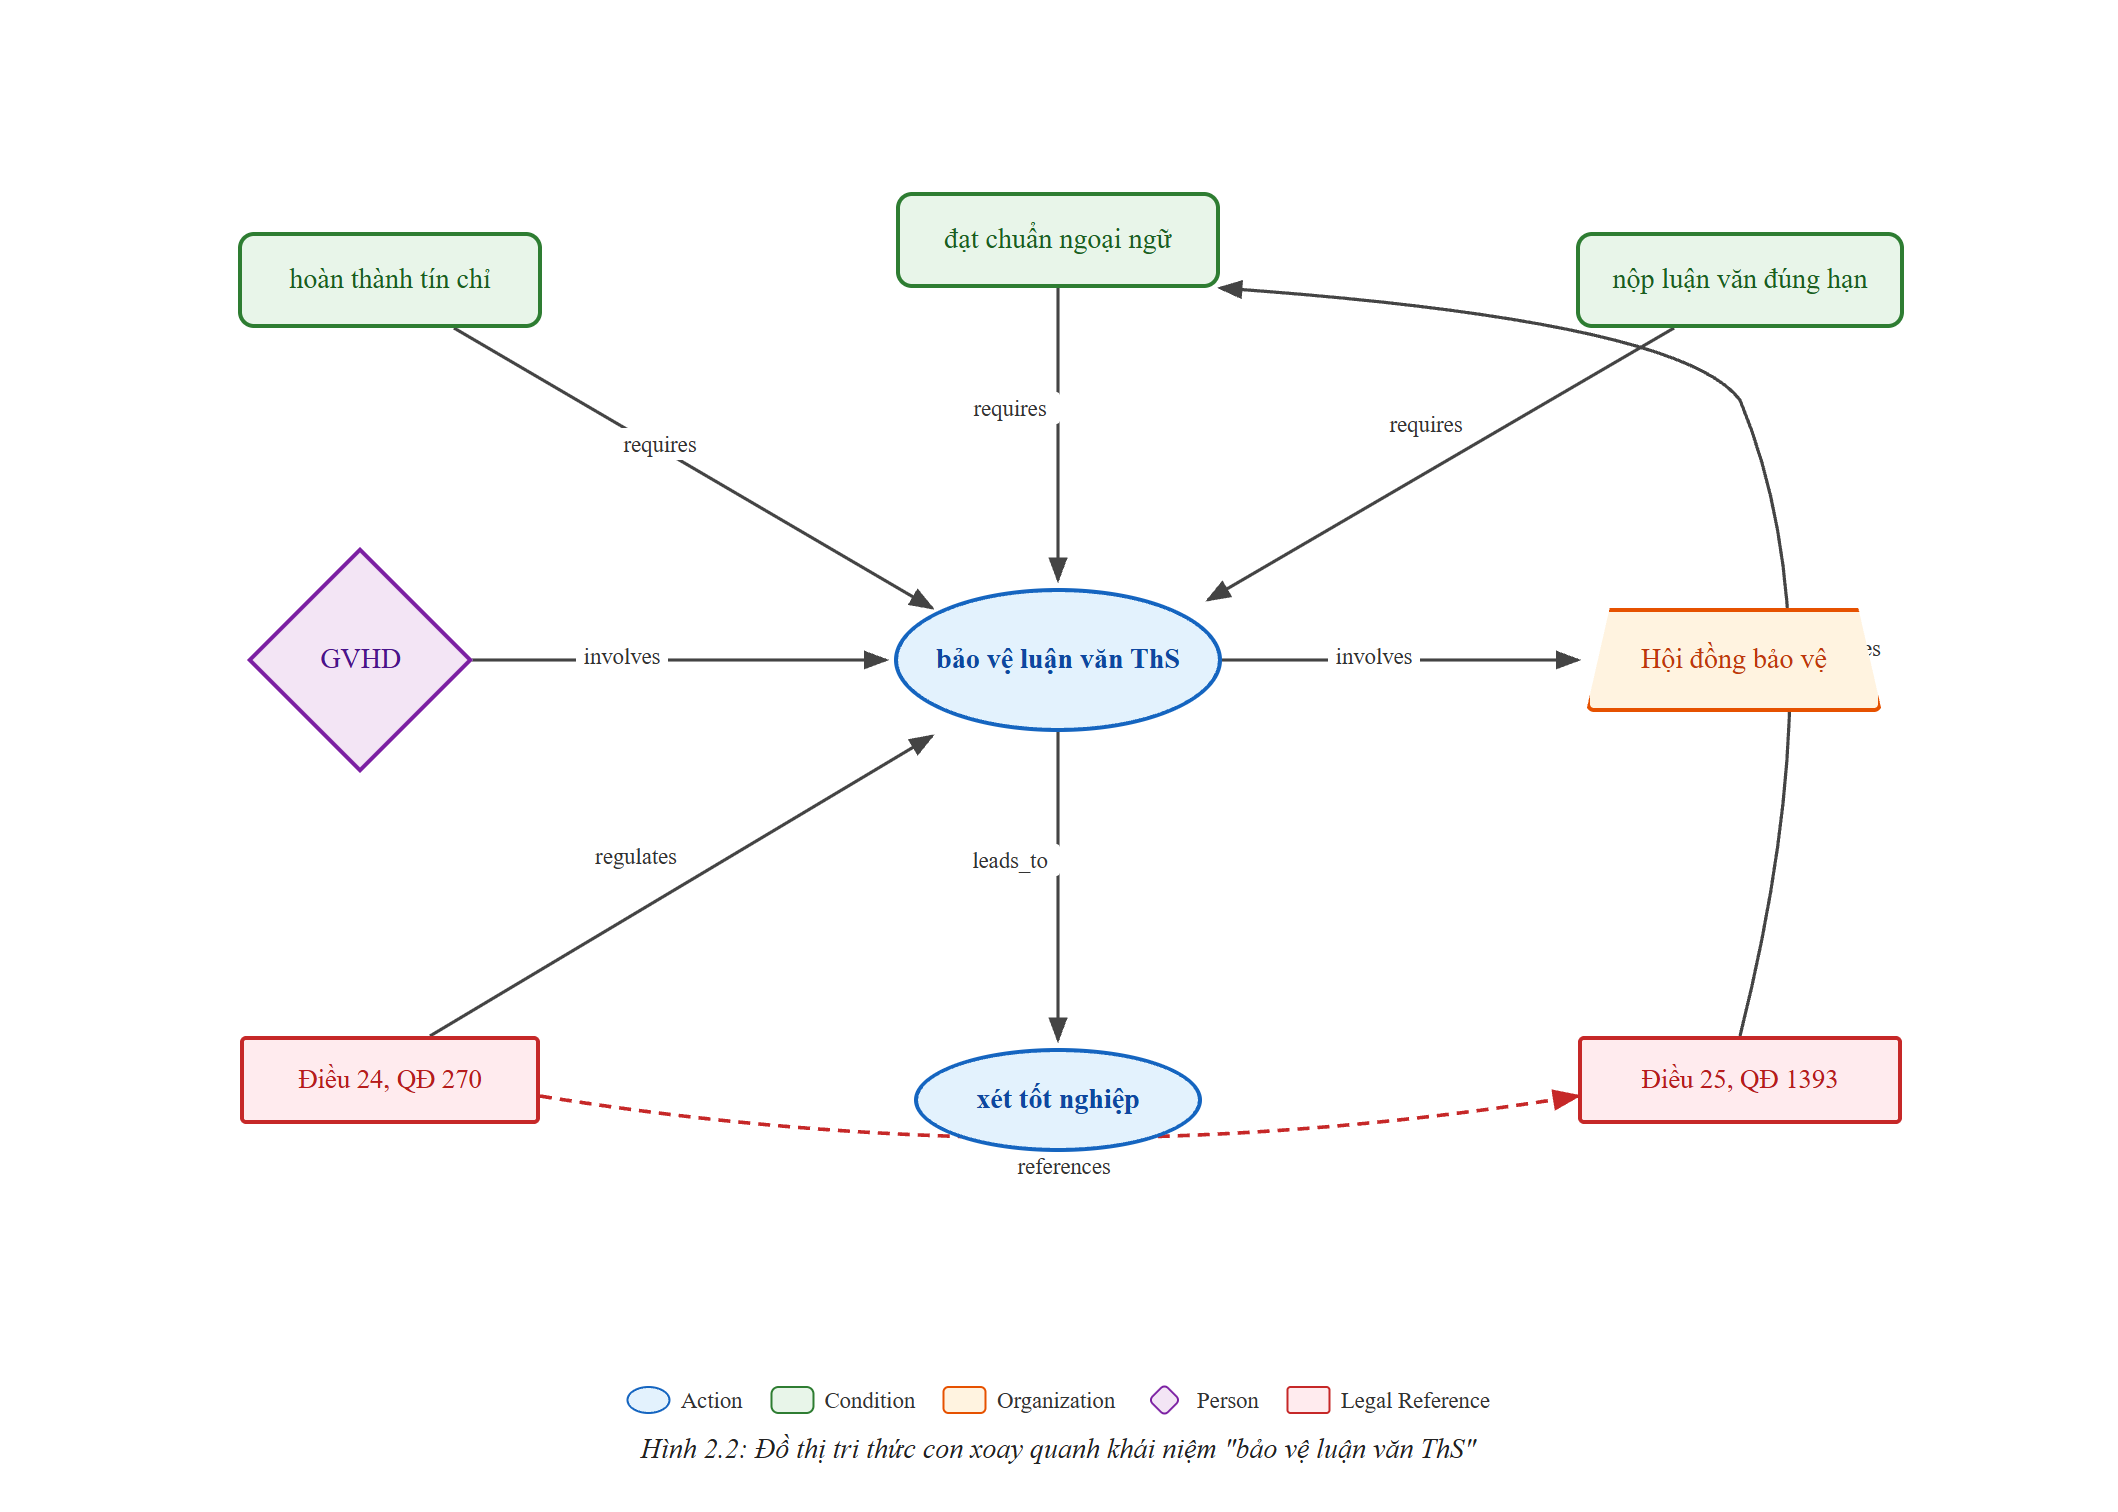
\includegraphics[width=0.95\textwidth]{graphics/figure2-2-kg-subgraph.png}
    \caption{Đồ thị con minh họa các thực thể và quan hệ xung quanh chủ đề ``bảo
    vệ luận văn thạc sĩ''. Các nút được phân loại theo ontology (Action, Condition,
    Organization, Person, Legal Reference) và các cạnh thể hiện các loại quan hệ
    (requires, leads\_to, regulates, references).}
    \label{fig:kg_subgraph}
\end{figure}

% ------------------------------------------------------------
\subsection{Phân loại chủ đề}
\label{subsec:phanloa_chude}

Bảng~\ref{tab:chude_phanloa} trình bày các nhóm chủ đề chính được phân loại từ nội
dung quy chế. Phân loại này phục vụ hai mục đích: tổ chức bộ câu hỏi kiểm thử
theo chủ đề để đảm bảo độ bao phủ, và xây dựng nhóm miền (domain group) cho
bước chọn tài liệu trong Tầng 1 của pipeline truy xuất.

\begin{table}[htbp]
    \centering
    \caption{Phân loại chủ đề trong quy chế đào tạo thạc sĩ}
    \label{tab:chude_phanloa}
    \begin{tabular}{clp{5.5cm}c}
        \toprule
        \textbf{STT} & \textbf{Chủ đề} & \textbf{Nội dung chính} & \textbf{Số điều liên quan} \\
        \midrule
        1 & Quy trình đào tạo
          & Đăng ký môn học, lịch học, nghỉ phép, chuyển ngành & 18 \\
        2 & Điều kiện tốt nghiệp
          & Điểm TB, ngoại ngữ, bài báo, luận văn & 12 \\
        3 & Luận văn
          & Đề cương, GVHD, hội đồng, bảo vệ, chỉnh sửa & 22 \\
        4 & Đánh giá kết quả
          & Thang điểm, quy đổi, cảnh báo, buộc thôi học & 10 \\
        5 & Tuyển sinh
          & Điều kiện dự tuyển, hồ sơ, xét tuyển & 8 \\
        6 & Liêm chính
          & Đạo văn, gian lận, xử lý vi phạm & 8 \\
        7 & Quy định GVHD
          & Tiêu chuẩn, số lượng, trách nhiệm & 6 \\
        \midrule
        & \textbf{Tổng} & & \textbf{84} \\
        \bottomrule
    \end{tabular}
\end{table}

Cần lưu ý rằng tổng số điều liên quan (84) nhỏ hơn tổng số điều (109) vì một số
điều thuộc phần điều khoản chung (quy định phạm vi, đối tượng, hiệu lực) không
nằm trong chủ đề chuyên biệt nào. Ngược lại, một số điều có thể liên quan đến
nhiều chủ đề; ví dụ Điều 24 QĐ~270 (điều kiện bảo vệ luận văn) liên quan đến cả
chủ đề ``Luận văn'' và ``Điều kiện tốt nghiệp''.

% ============================================================
\section{Tiền xử lý dữ liệu}
\label{sec:tien-xu-ly-du-lieu}

Sau khi thu thập và số hóa các văn bản quy chế, dữ liệu thô cần trải qua một
chuỗi bước tiền xử lý trước khi được đưa vào hệ thống truy xuất. Mục tiêu của
giai đoạn này là đảm bảo chất lượng và nhất quán của dữ liệu, đồng thời chuyển
đổi văn bản thành các biểu diễn số phục vụ cho truy xuất vector. Các bước tiền
xử lý bao gồm chuẩn hóa văn bản, xử lý cấu trúc phân cấp, và chuẩn bị dữ liệu
cho bước lập chỉ mục.

% ------------------------------------------------------------
\subsection{Chuẩn hóa văn bản}
\label{subsec:chuan-hoa-van-ban}

Văn bản pháp lý tiếng Việt thu thập từ nhiều nguồn khác nhau thường chứa nhiều
vấn đề về định dạng và mã hóa cần được xử lý thống nhất. Bước đầu tiên là chuẩn
hóa Unicode, đảm bảo rằng các ký tự tiếng Việt có dấu thanh điệu được biểu diễn
nhất quán. Trong thực tế, cùng một ký tự như ``ộ'' có thể được mã hóa theo hai
cách: một ký tự tổng hợp (precomposed, dạng NFC) hoặc ký tự cơ bản kết hợp với
dấu kết hợp (combining mark, dạng NFD), dẫn đến sự không nhất quán khi so khớp
chuỗi và tính toán embedding. Hệ thống sử dụng chuẩn hóa NFD (Canonical
Decomposition) để phân tách ký tự tiếng Việt thành ký tự cơ bản và dấu kết hợp,
cho phép so sánh và khớp chuỗi ở mức ký tự cơ bản một cách nhất quán. Cách tiếp
cận này đặc biệt hữu ích khi cần so khớp fuzzy giữa các chuỗi có dấu thanh điệu
khác nhau hoặc thiếu dấu do lỗi OCR.

Tiếp theo là chuẩn hóa khoảng trắng và ký tự đặc biệt. Các văn bản PDF sau khi
trích xuất text thường chứa nhiều khoảng trắng liên tiếp, ký tự tab, dấu cách
không phân cách (non-breaking space, U+00A0), và ký tự xuống dòng thừa. Tất cả
các biến thể khoảng trắng này được chuẩn hóa về dấu cách đơn (U+0020). Đối với
các ký tự đặc biệt xuất hiện trong văn bản pháp lý như dấu gạch ngang dài (em
dash ---), dấu gạch ngang ngắn (en dash --), và các biến thể dấu ngoặc kép (``
và '' theo kiểu typography), chúng được ánh xạ về dạng ASCII chuẩn tương ứng để
tránh sự không nhất quán khi so khớp từ khóa.

Định dạng số trong văn bản quy chế cũng được chuẩn hóa. Các ngày tháng xuất
hiện với nhiều dạng khác nhau (``25/04/2022'', ``ngày 25 tháng 4 năm 2022'',
``25-4-2022'') được chuẩn hóa về dạng ``dd/mm/yyyy''. Số hiệu điều khoản như
``Điều~24'' hay ``điều 24'' được thống nhất viết hoa chữ ``Điều'' để hỗ trợ
trích xuất tham chiếu chéo. Các giá trị số học liên quan đến điểm số, tín chỉ,
và thời gian được giữ nguyên nhưng chuẩn hóa đơn vị (ví dụ: ``1,5 năm'' thay
vì ``một năm rưỡi'').

Một thách thức đặc thù khi xử lý văn bản từ PDF scan là các lỗi OCR, mặc dù đã
sử dụng LLM Vision OCR với độ chính xác cao. Các lỗi phổ biến bao gồm dấu thanh
điệu bị lệch vị trí (ví dụ: ``quyêt'' thay vì ``quyết'', ``hôi'' thay vì
``hội''), chữ cái bị nhận nhầm do hình dạng tương tự (``l'' và ``1'', ``O'' và
``0''), và khoảng cách giữa các ký tự bị mất (``đàotạo'' thay vì ``đào tạo'').
Để xử lý các lỗi này, luận văn áp dụng danh sách thay thế (correction dictionary)
được tổng hợp từ quá trình rà soát thủ công trên toàn bộ kết quả OCR. Danh sách
bao gồm các cặp \texttt{(chuỗi\_lỗi, chuỗi\_đúng)} phổ biến nhất, ưu tiên các lỗi
xuất hiện ở nhiều văn bản. Quá trình thay thế được thực hiện theo thứ tự độ dài
giảm dần (longest-match-first) để tránh thay thế sai trong trường hợp một chuỗi
lỗi là tiền tố của chuỗi lỗi khác.

% ------------------------------------------------------------
\subsection{Xử lý cấu trúc phân cấp}
\label{subsec:xu-ly-cau-truc}

Sau khi chuẩn hóa văn bản thô, bước tiếp theo là chuyển đổi dòng văn bản liên
tục thành cấu trúc phân cấp có tổ chức, phản ánh hệ thống 6 cấp của văn bản
quy phạm pháp luật Việt Nam (Văn bản $\rightarrow$ Chương $\rightarrow$ Mục
$\rightarrow$ Điều $\rightarrow$ Khoản $\rightarrow$ Điểm).

Việc phát hiện ranh giới câu (sentence boundary detection) trong văn bản pháp lý
tiếng Việt đặt ra thách thức riêng so với văn bản thông thường. Viết tắt chuyên
ngành như ``ThS.'', ``QĐ.'', ``Đ.'' (viết tắt của ``Điều''), ``Kh.'' (``Khoản'')
thường chứa dấu chấm nhưng không đánh dấu kết thúc câu. Tương tự, các điều
khoản được đánh số như ``1.'' hay ``a)'' đứng đầu dòng không phải là ranh giới
câu. Luận văn xây dựng danh sách viết tắt chuyên ngành pháp lý và hành chính (bao gồm
các viết tắt tổ chức, loại hình doanh nghiệp, cơ quan nhà nước, và loại văn bản
quy phạm) để loại trừ khỏi bộ phát hiện ranh giới câu, kết hợp với quy tắc ngữ
cảnh: dấu chấm theo sau bởi chữ thường tiếp theo không được tính là kết thúc câu.

Phân đoạn đoạn văn (paragraph segmentation) tuân theo cấu trúc phân cấp cụ thể
của từng văn bản. Bộ phân tích cú pháp (parser) nhận diện các dấu hiệu cấp độ
qua pattern matching với regex tiếng Việt, sau đó sử dụng thuật toán đẩy--kéo
(push--pop stack) để xây dựng cây phân cấp. Điều quan trọng là không phải văn
bản nào cũng sử dụng đủ 6 cấp; ví dụ QĐ~270 không có cấp Mục, và bộ phân tích
phải xử lý cả trường hợp này mà không gây lỗi phân cấp.

Một số văn bản quy chế còn chứa bảng biểu và phụ lục. Ví dụ, QĐ~270 có bảng
quy đổi điểm số (Phụ lục~I) và biểu mẫu đơn xin bảo lưu kết quả (Phụ lục~II).
Các bảng biểu được trích xuất riêng và lưu trữ dưới dạng metadata gắn với nút
văn bản tương ứng trong cây phân cấp. Nội dung bảng biểu không được đưa vào quá
trình embedding vì định dạng dạng bảng thường không phù hợp với mô hình embedding
văn bản, thay vào đó được cung cấp trực tiếp cho LLM khi cần thiết thông qua
cơ chế tra cứu chính xác (exact lookup).

Trích xuất metadata từ tiêu đề và phần mở đầu văn bản bao gồm: số hiệu quyết
định (ví dụ: ``270/QĐ-ĐHCNTT''), ngày ban hành, cơ quan ban hành, và ngày có
hiệu lực. Thông tin này được lưu trữ dưới dạng thuộc tính (attribute) của nút
gốc trong Document Forest, phục vụ cho bộ lọc (filter) khi truy xuất theo văn
bản hoặc theo thời gian hiệu lực.

Phát hiện và xử lý trùng lặp nội dung là một vấn đề thực tế khi làm việc với
bộ văn bản quy chế có mối quan hệ kế thừa. QĐ~1393 kế thừa phần lớn nội dung
từ QĐ~160, trong khi QĐ~218 sửa đổi bổ sung một số điều trong QĐ~1393. Để tránh
việc cùng một thông tin pháp lý xuất hiện nhiều lần trong chỉ mục và gây nhiễu
kết quả truy xuất, luận văn áp dụng bộ phát hiện trùng lặp dựa trên độ tương
đồng chuỗi: mỗi điều khoản được chuẩn hóa về dạng canonical (loại bỏ dấu thanh
điệu, viết thường, chuẩn hóa viết tắt) và so sánh bằng Jaro-Winkler similarity.
Các điều khoản có độ tương đồng Jaro-Winkler $\geq 0{,}98$ được đánh dấu là
trùng lặp tiềm năng và xử lý theo chính sách ``giữ bản mới nhất''
(keep-latest): trong bộ dữ liệu này, ưu tiên QĐ~1393 so với QĐ~160 và QĐ~218
so với QĐ~1393 cho các điều khoản tương ứng.

% ------------------------------------------------------------
\subsection{Chuẩn bị dữ liệu cho truy xuất}
\label{subsec:chuan-bi-du-lieu}

Sau khi văn bản đã được chuẩn hóa và phân cấu trúc, bước cuối cùng là chuyển
đổi thành các biểu diễn phù hợp với hệ thống truy xuất. Giai đoạn này bao gồm
ba công việc chính: xác định đơn vị truy xuất (retrieval unit), tính toán
embedding vector, và xây dựng chỉ mục tìm kiếm.

Chiến lược phân đoạn theo điều (article-level chunking) được áp dụng: mỗi Điều
trong văn bản quy chế trở thành một đơn vị truy xuất độc lập. Cách tiếp cận này
ưu việt hơn phân đoạn theo kích thước cố định (fixed-size chunking) \cite{manning2008ir}
theo nhiều phương diện. Thứ nhất, mỗi Điều trong văn bản pháp lý có ngữ nghĩa
trọn vẹn và ranh giới pháp lý rõ ràng -- đây là đơn vị trích dẫn trong thực
tiễn hành chính và pháp lý Việt Nam. Thứ hai, phân đoạn theo điều bảo toàn ngữ
cảnh đầy đủ của quy định: một Điều về ``điều kiện bảo vệ luận văn'' chứa tất
cả các Khoản và Điểm liên quan, không bị cắt đứt giữa chừng như có thể xảy ra
với fixed-size chunking. Thứ ba, kích thước của các Điều trong bộ dữ liệu này
khá đồng đều (trung bình 180 token, min 45, max 520 token), phù hợp với giới
hạn của mô hình embedding.

Mỗi đơn vị truy xuất được gán một định danh nút (node ID) theo sơ đồ phân cấp
với tiền tố cho từng cấp: \texttt{c} cho chương (chapter), \texttt{d} cho điều
(article), \texttt{k} cho khoản (clause), và chữ cái thường cho điểm (point).
Cụ thể, định danh điều có dạng \texttt{\{doc\_id\}:d\{số\_điều\}}, trong đó
\texttt{doc\_id} là mã văn bản theo số hiệu quyết định (ví dụ:
\texttt{270-QD-DHCNTT}). Ví dụ đầy đủ: \texttt{270-QD-DHCNTT:d24} xác định
duy nhất Điều~24 của QĐ~270/QĐ-ĐHCNTT. Đối với cấp thấp hơn, định danh được
nối tiếp: \texttt{270-QD-DHCNTT:d24:k1} cho Khoản~1 của Điều~24, và
\texttt{270-QD-DHCNTT:d24:k1:a} cho Điểm~a của Khoản~1 đó.
Sơ đồ này cho phép cả truy xuất theo vị trí (vị trí trong cây Document
Forest) lẫn tra cứu trực tiếp theo số hiệu điều khoản.

Việc tính toán embedding sử dụng mô hình \texttt{paraphrase-multilingual-MiniLM-L12-v2}
\cite{reimers2019sbert}, một mô hình trong họ Sentence-BERT được huấn luyện đa
ngôn ngữ trên 50 ngôn ngữ bao gồm tiếng Việt. Mô hình này được chọn vì ba lý
do: hỗ trợ tiếng Việt tốt nhờ dữ liệu huấn luyện đa ngôn ngữ; kích thước
compact (117 triệu tham số, 418 MB) phù hợp triển khai trên phần cứng hạn chế;
và chiều embedding 384 tạo vector đủ biểu diễn mà không quá lớn ảnh hưởng
đến hiệu suất tìm kiếm. Mỗi đơn vị truy xuất (một Điều) được biểu diễn bởi một
vector embedding duy nhất tính từ toàn bộ nội dung điều đó, bao gồm tiêu đề và
tất cả các khoản, điểm con.

Việc sinh tóm tắt cho từng chương và điều bằng LLM (Claude 3.5 Haiku) được thực
hiện song song trong giai đoạn này, phục vụ cho Tầng~1 của pipeline truy xuất
(đã trình bày chi tiết tại Mục~\ref{subsec:quytrinh_thuthap}). Tóm tắt không
được dùng để thay thế nội dung gốc mà bổ sung thêm biểu diễn ngữ nghĩa ngắn
gọn, giúp Tầng~1 xác định nhanh nhánh Document Forest cần duyệt.

Sau khi tính xong tất cả 109 embedding vector (một cho mỗi Điều trong 5 văn bản
quy chế), các vector này được lưu trữ để phục vụ truy xuất ngữ nghĩa tại
Tầng~2 của pipeline. Việc tìm kiếm điều khoản tương đồng sử dụng cosine
similarity trên các vector embedding, cho phép xếp hạng các điều khoản theo
mức độ liên quan ngữ nghĩa đến truy vấn. Với tập dữ liệu nhỏ (109 vector,
384 chiều), phương pháp tìm kiếm vét cạn (exhaustive search) đảm bảo kết quả
chính xác 100\% mà không cần sử dụng chỉ mục xấp xỉ, đồng thời chi phí tính
toán hoàn toàn chấp nhận được (dưới 1~ms cho mỗi truy vấn).

Riêng đối với chỉ mục chủ đề (theme index), hệ thống sử dụng FAISS (Facebook
AI Similarity Search) với cấu hình \texttt{IndexFlatIP} kết hợp chuẩn hóa L2
(tương đương cosine similarity) để lưu trữ và tìm kiếm nhanh các vector embedding
của chủ đề. Chỉ mục FAISS cho chủ đề được lưu trữ dưới dạng nhị phân trên đĩa,
cho phép tải lại nhanh mà không cần tính toán lại embedding khi khởi động hệ thống.

Bảng~\ref{tab:thongke_tienxuly} tóm tắt các số liệu thống kê của bộ dữ liệu
sau khi hoàn tất quá trình tiền xử lý.

\begin{table}[htbp]
    \centering
    \caption{Thống kê dữ liệu sau tiền xử lý}
    \label{tab:thongke_tienxuly}
    \begin{tabular}{lr}
        \toprule
        \textbf{Thành phần} & \textbf{Số lượng/Giá trị} \\
        \midrule
        Tổng số điều khoản (retrieval units) & 109 \\
        Chiều embedding & 384 \\
        Mô hình embedding & MiniLM-L12-v2 \\
        Kích thước FAISS index & $\approx$ 167 KB \\
        Số nút Document Forest & 9.226 \\
        Tóm tắt chương & 17 \\
        Tóm tắt điều & 109 \\
        \bottomrule
    \end{tabular}
\end{table}

% ============================================================
\section{Thu thập câu hỏi kiểm thử}
\label{sec:cau_hoi_kiem_thu}

% ------------------------------------------------------------
\subsection{Nguồn thu thập và phương pháp}
\label{subsec:nguon_thuthap}

Tổng cộng 530 câu hỏi kiểm thử được thu thập từ hai nguồn: các nhóm tư vấn pháp
lý trên Facebook (400 câu hỏi pháp luật) và các diễn đàn học viên UIT (130 câu
hỏi quy định đào tạo). Các câu hỏi bao phủ nhiều mức độ phức tạp, từ tra
cứu đơn điều khoản (``Vốn điều lệ tối thiểu công ty chứng khoán là bao nhiêu?'')
đến các tình huống multi-hop đòi hỏi suy luận liên văn bản.

Mỗi câu hỏi được gán nhãn thủ công (manual annotation) bởi chuyên gia miền với
1--8 điều khoản liên quan (gold articles). Tiêu chí gán nhãn: một điều khoản được
gán là ``gold'' nếu cần thiết để trả lời đầy đủ câu hỏi -- tức là nếu thiếu điều
khoản đó, câu trả lời sẽ không hoàn chỉnh hoặc thiếu căn cứ.

Cụ thể, 400 câu hỏi pháp luật thuộc hai lĩnh vực: luật doanh nghiệp (200 câu,
Luật Doanh nghiệp 2020 và các nghị định hướng dẫn) và luật giao thông (200 câu,
Luật Trật tự, An toàn Giao thông Đường bộ 2024 và Nghị định 168/2024/NĐ-CP về
xử phạt vi phạm hành chính). 130 câu hỏi đào tạo bao gồm các chủ đề thường gặp
của học viên cao học: quy trình đào tạo, điều kiện tốt nghiệp, thủ tục bảo vệ luận
văn, chuẩn ngoại ngữ đầu ra, đăng ký môn học, và học phí. Việc đánh giá trên cả
ba miền nhằm chứng minh tính tổng quát của phương pháp.

% ------------------------------------------------------------
\subsection{Phân loại câu hỏi theo độ phức tạp}
\label{subsec:phanloa_cauhoi}

Bộ câu hỏi được phân loại theo ba mức độ phức tạp truy xuất, phản ánh số bước suy
luận cần thiết để tìm đúng điều khoản:

\begin{itemize}
    \item \textbf{Single-hop (58 câu, 44,6\%):} Câu hỏi chỉ cần tra cứu một điều
          khoản duy nhất, thường có từ khóa trùng khớp trực tiếp với tiêu đề hoặc
          nội dung điều khoản. Ví dụ: ``Thời gian đào tạo thạc sĩ tối đa là bao
          lâu?'' $\to$ Điều 5 QĐ~270 (thời gian đào tạo).

    \item \textbf{Multi-hop (52 câu, 40,0\%):} Câu hỏi cần kết hợp thông tin từ
          nhiều điều khoản hoặc nhiều văn bản. Chia thành hai dạng phụ:
          \begin{itemize}
            \item \textit{Intra-document} (31 câu): Nhiều điều trong cùng văn bản.
                  Ví dụ: ``Quy trình bảo vệ luận văn từ A-Z?'' cần Điều 22
                  (đề cương), Điều 23 (hội đồng), Điều 24 (điều kiện), Điều 25
                  (quy trình bảo vệ) QĐ~270.
            \item \textit{Cross-document} (21 câu): Kết hợp nhiều văn bản. Ví dụ:
                  ``Yêu cầu ngoại ngữ đầu ra cho học viên cao học?'' cần Điều 29
                  QĐ~270 (điều kiện tốt nghiệp) và Điều 25 QĐ~1393 (chi tiết yêu
                  cầu ngoại ngữ).
          \end{itemize}

    \item \textbf{Reasoning (20 câu, 15,4\%):} Câu hỏi đòi hỏi suy luận logic dựa
          trên các quy định, thường là tình huống giả định yêu cầu áp dụng nhiều
          điều kiện. Ví dụ: ``Học viên đã hết thời gian gia hạn nhưng chưa bảo vệ
          luận văn thì có thể làm gì?'' cần suy luận từ Điều 17 (gia hạn) kết hợp
          Điều 20 (buộc thôi học) và Điều 16 (bảo lưu).
\end{itemize}

% ------------------------------------------------------------
\subsection{Thống kê và phân tích bộ câu hỏi}
\label{subsec:thongke_cauhoi}

Bảng~\ref{tab:thongke_cauhoi} trình bày phân bố câu hỏi theo chủ đề. Phân bố này
phản ánh tần suất thực tế của các câu hỏi từ diễn đàn: quy trình đào tạo và điều
kiện tốt nghiệp là hai chủ đề được quan tâm nhiều nhất.

\begin{table}[htbp]
    \centering
    \caption{Thống kê bộ câu hỏi kiểm thử miền quy định đào tạo}
    \label{tab:thongke_cauhoi}
    \begin{tabular}{lccccc}
        \toprule
        \textbf{Chủ đề} & \textbf{Số câu} & \textbf{Tỷ lệ}
          & \textbf{Single} & \textbf{Multi} & \textbf{Reason} \\
        \midrule
        Quy trình đào tạo       & 28 & 21,5\% & 10 & 14 & 4 \\
        Điều kiện tốt nghiệp    & 25 & 19,2\% &  8 & 12 & 5 \\
        Luận văn                & 22 & 16,9\% &  8 & 10 & 4 \\
        Đánh giá kết quả        & 18 & 13,8\% & 12 &  4 & 2 \\
        Tuyển sinh              & 15 & 11,5\% &  9 &  4 & 2 \\
        Liêm chính học thuật    & 12 &  9,2\% &  6 &  4 & 2 \\
        Quy định GVHD           & 10 &  7,7\% &  5 &  4 & 1 \\
        \midrule
        \textbf{Tổng}           & \textbf{130} & \textbf{100\%}
          & \textbf{58} & \textbf{52} & \textbf{20} \\
        \bottomrule
    \end{tabular}
\end{table}

Phân tích cho thấy các chủ đề phức tạp (Luận văn, Điều kiện tốt nghiệp) có tỷ lệ
câu hỏi multi-hop và reasoning cao hơn do bản chất liên kết nhiều điều khoản. Ngược
lại, các chủ đề rõ ràng (Đánh giá kết quả, Tuyển sinh) có nhiều câu single-hop hơn.

Số gold articles trung bình mỗi câu hỏi là 3,0 (min: 1, max: 6, trung vị: 3). Phân
bố: 3 câu có 1 gold article, 40 câu có 2 gold articles, 49 câu có 3 gold articles,
29 câu có 4 gold articles, 8 câu có 5 gold articles, và 1 câu có 6 gold articles.
Phân bố nghiêng về phía đa điều khoản phản ánh đặc trưng tham chiếu chéo của hệ
thống quy chế đào tạo, nơi hầu hết câu hỏi đòi hỏi kết hợp quy định từ nhiều
điều khoản hoặc nhiều văn bản khác nhau.

Bảng~\ref{tab:vidu_cauhoi} trình bày 10 ví dụ câu hỏi mẫu từ bộ kiểm thử, bao
phủ các mức độ phức tạp và chủ đề khác nhau.

\begin{table}[htbp]
    \centering
    \caption{Ví dụ câu hỏi mẫu từ bộ kiểm thử}
    \label{tab:vidu_cauhoi}
    \begin{tabular}{ccp{6.5cm}p{3cm}}
        \toprule
        \textbf{STT} & \textbf{Loại} & \textbf{Câu hỏi} & \textbf{Gold articles} \\
        \midrule
        1  & S & Thời gian đào tạo thạc sĩ tối đa là bao lâu?
           & QĐ270: Đ.5 \\
        2  & M & Điều kiện để được bảo vệ luận văn thạc sĩ?
           & QĐ270: Đ.24; QĐ1393: Đ.25 \\
        3  & S & Điểm TB tích lũy tối thiểu để tốt nghiệp?
           & QĐ270: Đ.29 \\
        4  & M & Yêu cầu ngoại ngữ đầu ra cho học viên cao học?
           & QĐ1393: Đ.25; QĐ270: Đ.29 \\
        5  & S & Tiêu chuẩn để được làm GVHD luận văn ThS?
           & QĐ218: Đ.3 \\
        6  & S & Thế nào là hành vi đạo văn trong luận văn?
           & QĐ851: Đ.3 \\
        7  & S & Học viên bị cảnh báo học vụ khi nào?
           & QĐ270: Đ.18 \\
        8  & R & HV khóa 2021 có được áp dụng quy chế mới không?
           & QĐ1393: Đ.32 \\
        9  & M & Số tín chỉ tối thiểu cho ThS nghiên cứu?
           & QĐ270: Đ.8; QĐ1393: Đ.15 \\
        10 & R & GVHD được hướng dẫn tối đa bao nhiêu HV?
           & QĐ218: Đ.4 \\
        \bottomrule
    \end{tabular}
\end{table}

\noindent\textit{Ký hiệu: S = Single-hop, M = Multi-hop, R = Reasoning.}

Chi tiết kết quả đánh giá trên cả hai bộ dữ liệu (đào tạo và pháp luật) được trình
bày trong Chương~\ref{chap:chapter4}.
